% Last update: 17/08/2024

% Chú ý: đọc các phần chú ý đóng khung của file này và chỉnh lại cho phù hợp.

\documentclass[twoside,a4paper,14pt,openright]{extreport}
% font size
\usepackage[fontsize=13pt]{scrextend}
% Font tiếng Việt
\usepackage[T5]{fontenc}
\usepackage[utf8]{inputenc}
\DeclareTextSymbolDefault{\DH}{T1}

\usepackage{placeins} % Add this package

% Tài liệu tham khảo
\usepackage[
	sorting=nty,
	backend=bibtex,
	defernumbers=true]{biblatex}
\usepackage[unicode]{hyperref} % Bookmark tiếng Việt
\addbibresource{References/references.bib}

\makeatletter
\def\blx@maxline{77}
\makeatother

% Chèn hình, các hình trong luận văn được để trong thư mục Images/
\usepackage{graphicx}
\graphicspath{ {Images/} }
\usepackage{caption}
\usepackage[export]{adjustbox}

% Chèn và định dạng mã nguồn
\usepackage{listings}
\usepackage{color}
\usepackage{xcolor}
\definecolor{codegreen}{rgb}{0,0.6,0}
\definecolor{codegray}{rgb}{0.5,0.5,0.5}
\definecolor{codepurple}{rgb}{0.58,0,0.82}
\definecolor{backcolour}{rgb}{0.95,0.95,0.92}
\lstdefinestyle{mystyle}{
    backgroundcolor=\color{backcolour},   
    commentstyle=\color{codegreen},
    keywordstyle=\color{magenta},
    numberstyle=\tiny\color{codegray},
    stringstyle=\color{codepurple},
    basicstyle=\footnotesize,
    breakatwhitespace=false,         
    breaklines=true,                 
    captionpos=b,                    
    keepspaces=true,                 
    numbers=left,                    
    numbersep=5pt,                  
    showspaces=false,                
    showstringspaces=false,
    showtabs=false,                  
    tabsize=2
}
\lstset{style=mystyle}

% Chèn và định dạng mã giả
\usepackage{amsmath}
\usepackage{algorithm}
\usepackage[noend]{algpseudocode}
\makeatletter
\def\BState{\State\hskip-\ALG@thistlm}
\makeatother

% Bảng biểu
\usepackage{multirow}
\usepackage{array}
\newcolumntype{L}[1]{>{\raggedright\let\newline\\\arraybackslash\hspace{0pt}}m{#1}}
\newcolumntype{C}[1]{>{\centering\let\newline\\\arraybackslash\hspace{0pt}}m{#1}}
\newcolumntype{R}[1]{>{\raggedleft\let\newline\\\arraybackslash\hspace{0pt}}m{#1}}

% Đổi tên mặc định
\renewcommand{\chaptername}{CHƯƠNG}
\renewcommand{\figurename}{Hình}
\renewcommand{\tablename}{Bảng}
\renewcommand{\contentsname}{MỤC LỤC}
\renewcommand{\listfigurename}{DANH SÁCH CÁC HÌNH}
\renewcommand{\listtablename}{DANH SÁCH CÁC BẢNG}
\renewcommand{\appendixname}{PHỤ LỤC}

% Định dạng chapter
\usepackage{titlesec}

% Chỉ đánh số tới độ sâu là 3
\setcounter{secnumdepth}{3}

\titleformat{\chapter}
    [block]
    {\filcenter\normalfont\bfseries\normalsize}{\chaptername \ \thechapter :}{10pt}{\normalsize}
\titlespacing*{\chapter}{0pt}{-10pt}{10pt} %khoảng cách giữa chapter và đầu trang

\titleformat{\section}
    {\normalfont\bfseries\normalsize}{\thesection}{1em}{}
 
\titleformat{\subsection}
    {\normalfont\bfseries\normalsize}{\thesubsection}{1em}{}

\titleformat{\subsubsection}
    {\normalfont\bfseries\normalsize}{\thesubsubsection}{1em}{}

% Dãn dòng 1.5
\usepackage{setspace}
\onehalfspacing

% Thụt vào đầu dòng
\usepackage{indentfirst}

% Bottom right page numbering
\usepackage{fancyhdr} % for use of \pageref{LastPage}
\pagestyle{fancy} % Turn on the style
\fancyhf{} % Start with clearing everything in the header and footer
% Set the right side of the footer to be the page number
\fancyfoot[R]{\thepage}
\renewcommand{\headrulewidth}{0pt}%
% Redefine plain style, which is used for titlepage and chapter beginnings
% From https://tex.stackexchange.com/a/30230/828
\fancypagestyle{plain}{%
    \renewcommand{\headrulewidth}{0pt}%
    \fancyhf{}%
    \fancyfoot[R]{\thepage}%
}

% Canh lề
\usepackage[
  twoside,
  top=20mm,
  bottom=20mm,
  left=25mm,
  right=20mm,
  footskip = 15mm,
  includefoot]{geometry}

% Trang bìa
\usepackage{tikz}
\usetikzlibrary{calc}
\newcommand\HRule{\rule{\textwidth}{1pt}}

% Danh sách chữ viết tắt
\usepackage{myacronyms}

% ifelse
\usepackage{ifthen}

\newcommand\myemptypage{
\newpage
\thispagestyle{empty}
\mbox{}
\newpage
}

\usepackage[inkscapelatex=false]{svg}
\usepackage{tikz-timing}

\usepackage{booktabs}   % Cho bảng đẹp hơn
\usepackage{subcaption} % Cho hình ảnh con (subfigure)
% ========================================================================================= %
% CHÚ Ý: Thông tin chung về KLTN - sinh viên điền vào đây để tự động update các trang khác  %
% ========================================================================================= %
\newcommand{\displayTenSV}[1]{#1} % Dấu ~ là khoảng trắng không được tách (các chữ nối với nhau bằng dấu ~ sẽ nằm cùng 1 dòng
\newcommand{\tenKL}{Thiết~kế~và~Tích~hợp~Bộ~điều~khiển DMA~Tùy~chỉnh~trên~FPGA trong~Hệ~thống~SoC~Nios~V/m} % Chú ý dấu ~ trong tên khóa luận
\newcommand{\tenGVHD}{TS.~Huỳnh~Hữu~Thuận}
\newcommand{\tenBM}{}
\newcommand{\locationdateauto}[1]{Tp. #1, tháng \ifnum\month<10 0\fi\the\month/\the\year}
\begin{document}

% fix anchor bug
\hypersetup{pageanchor=false}
\begin{titlepage}

\begin{center}
ĐẠI HỌC QUỐC GIA THÀNH PHỐ HỒ CHÍ MINH\\
TRƯỜNG ĐẠI HỌC KHOA HỌC TỰ NHIÊN\\
\textbf{KHOA ĐIỆN TỬ - VIỄN THÔNG}\\[2cm]


{ \Large \bfseries \displayTenSV{MSSV~21207001 \\ Bùi~Thành~Đạt} \\[2cm] } 

%Tên đề tài Khóa luận tốt nghiệp/Đồ án tốt nghiệp
{ \Large \bfseries \textbf{BÁO CÁO THỰC TẬP THỰC TẾ} \\[3cm]} 


%Chọn trong các dòng sau
%\large KHÓA LUẬN TỐT NGHIỆP CỬ NHÂN\\
%\large ĐỒ ÁN TỐT NGHIỆP CỬ NHÂN\\
%\large THỰC TẬP TỐT NGHIỆP CỬ NHÂN\\
%\large BÁO CÁO THỰC TẬP THỰC TẾ\\
\large \tenKL \\ 
\large \text{} \\ 
\large \text{} \\
\large NGÀNH KỸ THUẬT ĐIỆN TỬ - VIỄN THÔNG\\
%Đưa vào dòng này nếu thuộc chương trình Chất lượng cao, hoặc lớp Cử nhân tài năng
% \large CHƯƠNG TRÌNH CHÍNH QUY\\
\large CHƯƠNG TRÌNH CHẤT LƯỢNG CAO\\
%\large CHƯƠNG TRÌNH CỬ NHÂN TÀI NĂNG\\[2cm]

\begin{tikzpicture}[remember picture, overlay]
  \draw[line width = 2pt] ($(current page.north west) + (2cm,-2cm)$) rectangle ($(current page.south east) + (-1.5cm,2cm)$);
\end{tikzpicture}

\vfill
\locationdateauto{Hồ Chí Minh}

\end{center}

\pagebreak

\myemptypage

\begin{center}
ĐẠI HỌC QUỐC GIA THÀNH PHỐ HỒ CHÍ MINH\\
TRƯỜNG ĐẠI HỌC KHOA HỌC TỰ NHIÊN\\
\textbf{KHOA ĐIỆN TỬ - VIỄN THÔNG}\\[2cm]


{\large \bfseries \displayTenSV{MSSV~21207001 \\ Bùi~Thành~Đạt} \\[2cm]}

%Tên đề tài Khóa luận tốt nghiệp/Đồ án tốt nghiệp
{ \Large \bfseries \textbf{BÁO CÁO THỰC TẬP THỰC TẾ} \\[2cm] } 


%Chọn trong các dòng sau
%\large KHÓA LUẬN TỐT NGHIỆP CỬ NHÂN\\
%\large ĐỒ ÁN TỐT NGHIỆP CỬ NHÂN\\
%\large THỰC TẬP TỐT NGHIỆP CỬ NHÂN\\
% \large BÁO CÁO THỰC TẬP THỰC TẾ\\
\tenKL
\large \text{} \\ 
\large \text{} \\
\large NGÀNH KỸ THUẬT ĐIỆN TỬ - VIỄN THÔNG\\
%Đưa vào dòng này nếu thuộc chương trình Chất lượng cao, hoặc lớp Cử nhân tài năng
% \large CHƯƠNG TRÌNH CHÍNH QUY\\
\large CHƯƠNG TRÌNH CHẤT LƯỢNG CAO\\[2cm]
%\large CHƯƠNG TRÌNH CỬ NHÂN TÀI NĂNG\\[2cm]

\textbf{GIÁO VIÊN HƯỚNG DẪN}\\
\tenGVHD

\begin{tikzpicture}[remember picture, overlay]
  \draw[line width = 2pt] ($(current page.north west) + (2cm,-2cm)$) rectangle ($(current page.south east) + (-1.5cm,2cm)$);
\end{tikzpicture}

\vfill
\locationdateauto{Hồ Chí Minh}

\end{center}
\thispagestyle{empty}

\myemptypage

\end{titlepage}
\hypersetup{pageanchor=true}
% Sau trang Title, các bạn chèn nhận xét gủa GVHD và GVPB. Nhận xét sẽ được giáo vụ phát sau buổi bảo vệ để các bạn đóng quyển.

\pagenumbering{roman} % Đánh số i, ii, iii, ...

%\addcontentsline{toc}{chapter}{Lời cam đoan}
%\include{Appendix/reassurances}
%\include{Appendix/editComfirmation}
%\include{Appendix/thanks}
%\include{Appendix/commitment}

%\chapter*{TÓM TẮT}
\label{Abstract}
\addcontentsline{toc}{chapter}{TÓM TẮT}

% Ngữ cảnh, vấn đề
Trong bối cảnh ngành thiết kế vi mạch, đặc biệt là thiết kế vi mạch số, đang ngày càng phát triển mạnh mẽ, việc hiểu rõ quy trình thiết kế trở nên vô cùng quan trọng.
% Mục tiêu
Báo cáo này trình bày quá trình thiết kế và đánh giá một mạch dịch 8-bit theo quy trình chuẩn của thiết kế vi mạch số, bao gồm lập trình Verilog, mô phỏng, tổng hợp mạch, kiểm tra \acrfull{drc} và \acrfull{lvs}.
% Phương pháp
Toàn bộ quy trình thiết kế được thực hiện thông qua bộ công cụ của Synopsys bao gồm \acrfull{vcs}, \acrfull{dc}, và \acrfull{icc2}. 
% Kết quả
Kết quả cuối cùng là một \acrfull{ip} mạch dịch 8-bit, có thể được sử dụng làm phần tử cơ bản trong các thiết kế lớn hơn.
% Kết luận
Bài báo cáo này khẳng định tầm quan trọng của việc nắm vững các quy trình thiết kế và công cụ hiện đại để đáp ứng nhu cầu ngày càng cao trong ngành công nghiệp vi mạch.

%\chapter*{ABSTRACT}
\label{Abstract-EN}
\addcontentsline{toc}{chapter}{ABSTRACT}

% Ngữ cảnh, vấn đề
In the era of revolutionary development in the semiconductor industry, particularly in the area of Digital \acrfull{ic} Design has been rapidly evolving, having comprehensive understanding of the design process has become increasingly critical.
% Mục tiêu
This report outlines the design and evaluation of an 8-bit shift register, complying with the standard Digital \acrshort{ic} Design procedures including Verilog programming, simulation, circuit synthesis, \acrfull{drc} and \acrfull{lvs} verification.
% Phương pháp
The entire design process was conducted using Synopsys toolsets, including \acrfull{vcs}, \acrfull{dc}, and \acrfull{icc2}. 
% Kết quả
The final outcome is an 8-bit shift register \acrfull{ip} that can be utilized as a basic building block in more complex designs.
% Kết luận
This report aims to underscore the importance of mastering modern tools and design methodologies to meet the increasing demands of the semiconductor industry.

% \phantomsection
% \addcontentsline{toc}{chapter}{Đề cương chi tiết}
% \include{Appendix/decuong}

% Mục lục, danh sách hình, danh sách bảng
\cleardoublepage
\phantomsection
\addcontentsline{toc}{chapter}{MỤC LỤC}
\tableofcontents
% Danh sách chữ viết tắt
\printglossary[type=\acronymtype,
                title=DANH SÁCH CHỮ VIẾT TẮT, 
                toctitle=DANH SÁCH CHỮ VIẾT TẮT
                ]

\cleardoublepage
\newpage
\phantomsection
\addcontentsline{toc}{chapter}{\listfigurename}
\listoffigures

\cleardoublepage
\newpage
\phantomsection
\addcontentsline{toc}{chapter}{\listtablename}
\listoftables

\cleardoublepage

\pagenumbering{arabic} % Đánh số 1, 2, 3, ...

% Các chương nội dung
% !TEX encoding = UTF-8 Unicode
% Ensure this file is saved with UTF-8 encoding

% \chapter{GIỚI THIỆU} % Keep this if it's the actual first chapter
% \label{Chapter1} % Keep label consistent if referenced elsewhere

% If this CESLAB intro is *part* of Chapter 1, use \section instead of \chapter
% Example:
\chapter{INTRODUCTION}
\label{Chapter1} % Label for the whole introduction chapter

% Problem Statement, Background, and Motivation
% The need for research

% Lưu ý: Đảm bảo đã thêm \usepackage{booktabs} và \usepackage{subcaption} vào main.tex
% Lưu ý: Cần chuẩn bị các file ảnh từ PDF và thêm các môi trường \begin{figure}...\end{figure} tương ứng.
\chapter{THEORETICAL FOUNDATION} % Revised Title
\label{Chapter2}

\section{Chipyard Framework}
\label{sec:chipyard}

\subsection{Overview of Chipyard}
\label{sec:chipyard_overview}
% \begin{figure}[htbp]
%     \centering
%     \includegraphics[width=0.8\textwidth]{figures/chipyard_overview.png}
%     \caption{Overview of the Chipyard Framework}
%     \label{fig:chipyard_overview}
% \end{figure}

Chipyard is an open-source System-on-Chip (SoC) design framework that facilitates the agile development of complex, customized hardware systems \cite{chipyard}. It provides an integrated environment that brings together a vast collection of \gls{rtl} (Register Transfer Level) generators, simulation tools, and implementation flows. The primary goal of Chipyard is to enable rapid architectural exploration, design, and evaluation of SoCs, particularly those incorporating specialized hardware accelerators and heterogeneous core configurations.

\subsection{Key Components of Chipyard}
\label{sec:chipyard_key_components}

\begin{itemize}
    \item \textbf{RTL Generators:} Chipyard leverages a rich library of open-source, generator-based IP blocks. These generators, primarily written in \gls{chisel} (Constructing Hardware In a Scala Embedded Language), allow for highly parameterized and composable hardware designs. This includes RISC-V cores (like Rocket and \gls{boom}), caches, interconnects, peripherals, and domain-specific accelerators \cite{chipyard}.

    \item \textbf{SoC Configuration:} Designs in Chipyard are specified through a powerful configuration system. Users can define the SoC architecture, select IP blocks, and customize their parameters without directly modifying the \gls{rtl} source code. This promotes modularity and reusability \cite[p.~27]{chipyard}.

    \item \textbf{FIRRTL Intermediate Representation:} Chisel designs are elaborated into \gls{firrtl} (Flexible Intermediate Representation for RTL). Chipyard utilizes \gls{firrtl} transformations to adapt the generated hardware for various downstream tools and flows, such as software simulation, \gls{fpga} emulation, and ASIC implementation \cite{chipyard}.

    \item \textbf{Simulation and Verification:} Chipyard supports multiple simulation methodologies:

    \begin{itemize}
        \item Software RTL Simulation: Cycle-accurate simulation using tools like Verilator or commercial simulators for detailed debugging and verification \cite[p.~29]{chipyard}.

        \item FPGA-Accelerated Simulation (FireSim): For faster, full-system validation with long-running workloads, Chipyard integrates FireSim. FireSim enables cycle-exact simulation on cloud-hosted \glspl{fpga}, providing a scalable and accessible platform for pre-silicon performance evaluation \cite{karandikar2018firesim, chipyard}. 

        \item VLSI Implementation (Hammer): For physical design, Chipyard includes Hammer, a VLSI flow that abstracts process-technology and EDA-tool specifics, enabling more portable and reusable physical design scripts \cite{chipyard}.

        \item Workload Management (FireMarshal): Chipyard provides FireMarshal for generating and managing software workloads, including Linux distributions, to run on the simulated or emulated hardware \cite{chipyard}.
    \end{itemize}
\end{itemize}

Chipyard's methodology promotes an agile hardware development process, allowing for iterative design, continuous integration, and validation of physically realizable custom \glspl{soc}. This research utilizes Chipyard as the foundational framework for constructing and evaluating the Rocket Chip-based \gls{soc} with the Gemmini accelerator.

\section{Rocket Chip and RISC-V}
\label{sec:rocketchip_riscv}

The foundation of the processing system developed in this thesis lies in the RISC-V instruction set architecture and its implementation through the Rocket Chip SoC generator.

\subsection{The RISC-V Instruction Set Architecture (ISA)}
\label{sec:riscv_isa}

The RISC-V ISA represents a paradigm shift in processor design, moving away from proprietary, closed architectures towards a free and open standard. This openness is a crucial enabler for innovation, allowing researchers, academics, and industry professionals to design, implement, and extend processor architectures without restrictive licensing fees or access limitations \cite{asanovic2014riscv}. RISC-V is designed with simplicity, modularity, and extensibility at its core.

Key characteristics of the RISC-V ISA relevant to this work include:
\begin{itemize}
    \item \textbf{Modularity:} The ISA is defined as a small base integer instruction set (e.g., RV32I for 32-bit, RV64I for 64-bit systems) with multiple standard optional extensions that can be added to meet specific application needs. This thesis focuses on an RV64I base. Common extensions include 'M' for integer multiplication and division, 'A' for atomic instructions, 'F' for single-precision floating-point, 'D' for double-precision floating-point, and 'C' for compressed instructions. The combination of IMAFD is often referred to as 'G' for general-purpose computing \cite{asanovic2016rocketchip}.

    \item \textbf{Extensibility:} RISC-V reserves a significant portion of its opcode space for custom, non-standard extensions. This allows for the tight integration of specialized hardware, such as the Gemmini accelerator used in this research, directly into the processor's instruction set if desired, or via coprocessor interfaces.

    \item \textbf{Privileged Architecture:} To support complex operating systems like Linux, RISC-V defines a privileged architecture with multiple modes of operation, including Machine (M), Supervisor (S), and User (U) modes. The Supervisor mode, along with mechanisms for virtual memory management (Memory Management Unit - MMU) and interrupt handling, is essential for OS functionality \cite{waterman2015riscvpriv}.

    \item \textbf{Growing Ecosystem:} The open nature of RISC-V has fostered a rapidly expanding ecosystem of compatible cores, development tools (compilers like GCC and LLVM, simulators like Spike and QEMU), and operating system ports (including Linux and FreeBSD).
\end{itemize}

\subsection{Rocket Chip SoC Generator}
\label{sec:rocketchip_generator}

Rocket Chip is a highly influential open-source SoC generator that produces synthesizable RTL for systems based on the RISC-V ISA \cite{asanovic2016rocketchip}. It is a cornerstone of the Chipyard framework and is itself developed using Chisel. Instead of being a fixed processor design, Rocket Chip is a generator capable of producing a wide variety of SoC configurations, from simple microcontrollers to complex multi-core systems capable of running full operating systems.

Key aspects of the Rocket Chip generator utilized or relevant to this thesis include:
\begin{itemize}
    \item \textbf{Core Generators:}
    \begin{itemize}
        \item Rocket Core: This is a highly configurable, in-order, scalar RISC-V core generator. It can be parameterized to implement various ISA subsets (e.g., RV64G as used in this project). Crucially for this research, it features a sophisticated Memory Management Unit (MMU) supporting page-based virtual memory, configurable branch prediction mechanisms, and non-blocking data caches. These features, along with its support for Supervisor mode, make it well-suited for running operating systems like Linux \cite[p.~4]{asanovic2016rocketchip}. This is the primary core utilized in this thesis.

        \item BOOM (Berkeley Out-of-Order Machine): Rocket Chip also includes a generator for BOOM, an out-of-order, superscalar core designed for higher performance applications, demonstrating the generator's versatility \cite[p.~5]{asanovic2016rocketchip}.
    \end{itemize}

    \item \textbf{Cache Hierarchy:} The generator provides configurable L1 instruction and data caches for each core, as well as an optional shared L2 cache. Parameters such as cache size, associativity, number of banks, and replacement policies can be customized to explore different points in the design space \cite[p.~3]{asanovic2016rocketchip}.

    \item \textbf{TileLink Interconnect:} Rocket Chip employs TileLink, an open-source, chip-scale interconnect protocol designed to connect various components within the SoC, including cores, caches, memory controllers, and peripherals. TileLink supports cache coherence, enabling the construction of complex, coherent multi-core systems and accelerator integrations \cite[p.~6]{asanovic2016rocketchip} \cite[p.~15]{chipyard}.

    \item \textbf{RoCC (Rocket Custom Coprocessor) Interface:} This standardized interface facilitates the integration of custom hardware accelerators, termed RoCC accelerators, with Rocket or BOOM cores. Accelerators connected via RoCC can be issued custom instructions decoded by the core, can access core registers, and can interact with the memory system. They can share the core's L1 data cache and Page Table Walker (PTW) for virtual memory support, or connect directly to the TileLink fabric for higher bandwidth memory access \cite[p.~5]{asanovic2016rocketchip} \cite[p.~13]{chipyard}. The Gemmini accelerator in this thesis is integrated using this interface.
\end{itemize}

This research specifically leverages the Rocket core generator within the Chipyard framework to construct a 64-bit RISC-V system (based on the Rocket64b1gem16 configuration), which is then targeted for implementation and evaluation on a Xilinx VC707 FPGA board.

\section{Gemmini Accelerator}
\label{sec:gemmini_accelerator}

Gemmini is a highly configurable, open-source systolic array-based matrix multiplication accelerator generator, designed to accelerate machine learning workloads, particularly deep neural networks \cite{genc2019gemmini, chipyard}. It is typically integrated into a Chipyard-based SoC as a RoCC accelerator, allowing it to be controlled by custom RISC-V instructions executed on a host core like Rocket.

Key Features of Gemmini:
\begin{itemize}
    \item \textbf{Systolic Array Architecture:} Gemmini employs a 2D systolic array of processing elements (PEs) to perform matrix multiplications efficiently. The dimensions of this array, dataflow (e.g., weight-stationary, output-stationary), and data types are configurable.

    \item \textbf{On-Chip Scratchpad Memory:} It includes dedicated on-chip SRAM (scratchpad memory) for storing input activations, weights, and partial sums, reducing reliance on off-chip memory bandwidth.

    \item \textbf{Configurability:} Gemmini offers extensive parameterization, allowing designers to explore a wide design space. This includes the systolic array dimensions, scratchpad memory sizes, data precision, and the interface to the memory system.

    \item \textbf{RoCC Integration:} As a RoCC accelerator, Gemmini can be issued commands by the CPU. These commands can configure the accelerator, load data into its scratchpads, and initiate matrix multiplication operations. It can leverage the CPU's virtual memory system through the RoCC interface for memory accesses \cite[p.~13]{chipyard}.
\end{itemize}

In this thesis, the Gemmini accelerator is integrated with the Rocket core to provide hardware acceleration for the matrix multiplication operations that are fundamental to many machine learning algorithms. The successful execution of tests from gemmini-rocc-tests confirms the functional integration of Gemmini within the built system.

\section{Linux on RISC-V SoCs}
\label{sec:linux_on_riscv}

Running a full-fledged operating system like Linux on a custom-designed RISC-V SoC involves several key software and hardware components working in concert. The ability to boot Linux signifies a mature and functional hardware platform capable of supporting complex software stacks. The project eugene-tarassov/vivado-risc-v, referenced in the current results, provides a specific environment and set of configurations for achieving this on a Xilinx VC707 board.

General components and processes involved include:
\begin{itemize}
    \item \textbf{RISC-V Privileged Architecture:} The RISC-V ISA includes a privileged architecture specification that defines different privilege modes (Machine, Supervisor, User), control and status registers (CSRs), and mechanisms for memory management (MMU) and interrupt handling. A Linux-capable core must implement the Supervisor mode and support virtual memory \cite{waterman2015riscvpriv}. Rocket Chip cores, like the one used, provide this support \cite{asanovic2016rocketchip}.

    \item \textbf{Bootloader:} A bootloader is the first piece of software that runs after system reset. Its primary role is to initialize the hardware (e.g., memory controller, console) and then load the operating system kernel into memory and transfer execution to it. Common bootloaders for RISC-V include:
    \begin{itemize}
        \item Berkeley Boot Loader (BBL): Often used with Rocket Chip, BBL can run in Machine mode and provides a Supervisor-mode execution environment for the Linux kernel. It typically includes a device tree blob.

        \item U-Boot: A more versatile and widely used bootloader that supports multiple architectures, including RISC-V.
    \end{itemize}

    \item \textbf{Device Tree (DTB):} The Device Tree Blob is a data structure passed to the kernel by the bootloader. It describes the hardware components of the system (e.g., number of cores, memory map, peripherals, interrupt controllers) in a standardized way, allowing the kernel to be hardware-agnostic to a certain extent.

    \item \textbf{Linux Kernel:} A port of the Linux kernel for the RISC-V architecture is required. This kernel must include drivers for the specific peripherals present in the SoC (e.g., UART for console, network interface, block device controller if present).

    \item \textbf{Root Filesystem:} Once the kernel is running, it mounts a root filesystem which contains the user-space applications, libraries, and system utilities that constitute the Linux distribution (e.g., Debian, Fedora, Buildroot).
\end{itemize}

The vivado-risc-v project likely provides pre-compiled versions or build scripts for these components, specifically tailored for the Rocket Chip configuration deployed on the VC707, including necessary FPGA-specific configurations (e.g., for DDR memory controller, Ethernet, UART through JTAG or physical pins). Successfully booting Debian Linux demonstrates that the custom SoC, including the Rocket core, memory system, and peripherals, are functioning correctly and are sufficiently robust to support a complex operating system.

\section{Time-Series Anomaly Detection}
\label{sec:time_series_anomaly}

This subsection will be elaborated upon once the machine learning model for arrhythmia time-series anomaly detection is developed and implemented. It will cover the theoretical underpinnings of the chosen anomaly detection algorithms, relevant time-series analysis techniques, and how these map to the capabilities of the Gemmini-accelerated RISC-V platform.

\chapter{A Multi-Core RISC-V Processor System}
\label{chap:MultiCoreRISCVSystem}

From the surveys and analyses in the preceding sections regarding processor cores and the two SoC development frameworks, it is evident that each of these research subjects possesses distinct advantages and limitations. However, for the research orientation and implementation of a processor system featuring a custom accelerator, the \texttt{Chipyard} framework and its library components are deemed most suitable for the objectives of this thesis. Not only does \texttt{Chipyard} effectively meet current requirements, but it also holds the potential for expansion to support more complex systems in the future.

This chapter will present a more detailed exposition of the component structure and the process of constructing an SoC system, while also delving into the architecture of the \texttt{Rocket} processor core. The thesis will utilize high-level design languages \texttt{Chisel}/\texttt{Scala} to implement a single-core processor system integrated with the \texttt{Gemmini} \texttt{RoCC} accelerator, focusing on leveraging the components within an SoC system, and building the hardware and software design based on the \texttt{Chipyard} framework.

\section{System Design Methodology with \texttt{Chisel}}
\label{sec:design_methodology_chisel}

As previously introduced, this thesis undertakes system design based on the components and tools within \texttt{Chipyard}. This framework and its library components are constructed from a diverse range of elements, all based on \texttt{Chisel}/\texttt{Scala}.

\subsection{\texttt{Chisel} and \texttt{Scala}}
\label{subsec:chisel_scala}

\begin{figure}[htbp]
    \centering
    \begin{subfigure}[b]{0.3\textwidth}
        \centering
        \includegraphics[width=\linewidth]{Images/Chisel_logo.pdf}
    \end{subfigure}%
    \hfill
    \begin{subfigure}[b]{0.18\textwidth}
        \centering
        
\includegraphics[width=\linewidth]{Images/Chisel_Scala_Logo.pdf}
    \end{subfigure}%
    \hfill
    \begin{subfigure}[b]{0.18\textwidth}
        \centering
        
\includegraphics[width=\linewidth]{Images/Chisel_FIRRTL.pdf}
    \end{subfigure}%
    \hfill
    \begin{subfigure}[b]{0.2\textwidth}
        \centering
        
\includegraphics[width=\linewidth]{Images/Chisel_ChipsAlliance.pdf}
    \end{subfigure}
    \caption{\texttt{Chisel} as a library within \texttt{Scala}. Source: CHIPS Alliance.}
    \label{fig:chisel_ecosystem_logos}
\end{figure}

\texttt{Chisel} is a Hardware Construction Language (HCL) developed at UC Berkeley, initially intended to enable hardware design through highly parameterized and hierarchically specific code generators. \texttt{Chisel} is used to define these generators, which then produce designs in \texttt{Verilog}, suitable for industry-standard RTL design flows. \texttt{Chisel} is classified as a Domain-Specific Language (DSL); more precisely, it is implemented as a library package for \texttt{Scala}, a high-level, multi-paradigm programming language that integrates features of both Object-Oriented Programming (OOP) and functional programming on the \texttt{Java} Virtual Machine (JVM). Furthermore, \texttt{Scala}'s functional programming capabilities support higher-order functions and immutable data structures, facilitating more maintainable code, which is crucial for reproducibility and collaboration in scientific research.

\texttt{Chisel}'s design aims to address the lack of object-oriented programming and pre-processing structures in existing Hardware Description Languages (HDLs), supporting the construction of more flexible generators. By being based on \texttt{Scala}, \texttt{Chisel} gains the flexibility to describe hardware with high levels of abstraction and modularity. This helps hardware designers describe circuits in a way that is easy to maintain, modify, and extend, especially for large and complex designs such as microprocessors and specialized digital signal processing cores. \texttt{Scala}'s robust type system, diverse numerical representations and variables, immutability, and support for functional programming make it an ideal foundation for \texttt{Chisel}, aiding in error checking during hardware and circuit description and encouraging reusable design patterns.

In the context of hardware design based on \texttt{Chisel} and \texttt{Scala}, \texttt{sbt} (Simple Build Tool) plays a crucial role, optimizing the design management and development process. Built specifically for \texttt{Scala} and \texttt{Java} projects, \texttt{sbt} is the build tool used by the majority of \texttt{Scala} developers. Essentially, \texttt{sbt} acts as the compiler when working with \texttt{Chisel} and \texttt{Scala}. Using \texttt{sbt} simplifies the process of structuring projects for hardware design with \texttt{Chisel} in \texttt{Chipyard}, as well as enabling integration with many other open-source projects.

\subsection{\texttt{Verilator} Simulation Tool}
\label{subsec:verilator}

In the hardware design process, evaluating the functionality of the design is critically important. With \texttt{Chipyard}, system designs, from simple to complex structures, can be effectively realized and tested thanks to integrated tools and RTL simulators like \texttt{Verilator}, which are readily available within the project framework.

\texttt{Verilator} is an open-source program, prominent in the field of RTL simulation due to its unique method of converting ("Verilating") \texttt{Verilog} or \texttt{SystemVerilog} into \texttt{C++} or \texttt{SystemC}, creating a highly optimized executable program. Unlike traditional simulators, \texttt{Verilator} does not directly interpret \texttt{Verilog} during simulation. Instead, it generates \texttt{C++} or \texttt{SystemC} program files by parsing the hardware code, performing syntax checking, linting, and optionally inserting debug points and coverage analysis to enhance the correctness and accuracy of evaluation and verification. This "Verilated" output file can be configured to run in single-threaded or multi-threaded mode on a development server, offering an advantage for simulating complex or computationally demanding designs. After the "Verilated" code is generated, it is compiled by a standard \texttt{C++} compiler such as \texttt{GCC}, \texttt{Clang}, or \texttt{MSVC++}, and is typically combined with a user-provided wrapper file to manage the initialization of the Verilated model.

\texttt{Verilator} offers high simulation performance, especially for designs requiring substantial resources, due to its high speed and cycle accuracy. \texttt{Verilator}'s compilation approach makes it up to 100 times faster than interpretive simulators like Icarus \texttt{Verilog} (which is also open-source), and with multi-threading, performance can increase by an additional 2-10 times, achieving a total improvement of up to 1000 times. This makes \texttt{Verilator} suitable for RISC-V multi-core processor designs ranging from simple to complex, and competitive even with commercial simulators such as Synopsys VCS, Cadence Incisive, or Mentor ModelSim.

\section{The \texttt{Rocket} Processor Core}
\label{sec:rocket_core}

As introduced in the previous chapter, \texttt{Rocket} is a 5-stage, in-order processor core compliant with the RISC-V instruction set architecture, with RV32G and RV64G variants. Currently, the development of the \texttt{Rocket} core is maintained by the CHIPS Alliance. \texttt{Rocket} is written in the \texttt{Chisel} hardware design language, based on the \texttt{Scala} programming language, and is a key component of the \texttt{Rocket Chip} SoC Generator toolchain.

When implemented, each \texttt{Rocket} core is combined with L1 data and instruction caches. This memory operates locally for each core and, in a multi-core system, is responsible for storing temporary variables generated during the execution of the pipeline, helping to reduce congestion when multiple cores attempt to store data. Together with the Page Table Walker (\texttt{PTW}), a Tile within the SoC is formed. This \texttt{Rocket} Tile (Figure \ref{fig:rocket_tile_structure}) is considered a fundamental unit in the \texttt{Rocket Chip} SoC system and can be replicated to create multi-core processor systems, meeting the demands for performance and flexibility in modern SoC design.

\begin{figure}[h!]
    \centering
    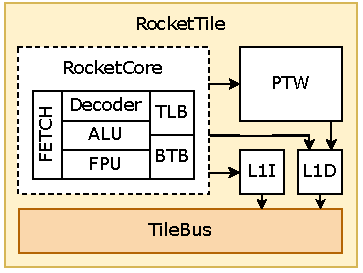
\includegraphics[width=0.7\textwidth]{Images/RocketTile_Basic.pdf}
    \caption{Structure of a \texttt{Rocket} Tile.}
    \label{fig:rocket_tile_structure}
\end{figure}

Due to the object-oriented nature of \texttt{Chisel}, the language used for its design, \texttt{Rocket} itself is written from object classes that can be defined and reconfigured according to implementation needs, such as \texttt{WithNBigCore()}, \texttt{WithNMedCore()}, \texttt{WithNSmallCore()}, and \texttt{WithNTinyCore()}. Additionally, instead of implementing the \texttt{Rocket} core, the \texttt{BOOM} core can also be integrated in its place, and many other peripherals can be integrated into a Tile unit.

\section{\texttt{Rocket Chip} SoC Structure}
\label{sec:rocketchip_soc_structure}

This system generator includes multiple components, not just the processor core but also the on-chip system bus (SoC bus), specifically \texttt{TileLink}. \texttt{TileLink} comprises a peripheral bus, control bus, and memory bus, along with arbiters and system controllers. Additionally, the system integrates peripheral components such as DRAM, GPIO, UART, and, critically for this thesis, supports tightly-coupled accelerators like \texttt{Gemmini} via the \texttt{RoCC} interface. Figure \ref{fig:single_core_gemmini_system} below depicts the generalized structure of the single-core RISC-V processor system with a \texttt{Gemmini} \texttt{RoCC} accelerator, which forms the basis for the development in this thesis.

\begin{figure}[h!]
    \centering
    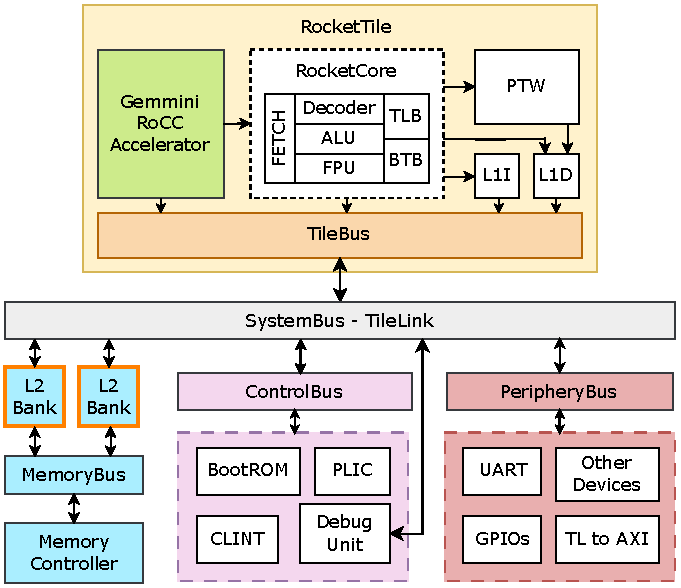
\includegraphics[width=0.9\textwidth]{Images/RocketChip_Gemmini_Diagram.pdf}
    \caption{Proposed structure of a single-core RISC-V processor system with a \texttt{Gemmini} \texttt{RoCC} accelerator.}
    \label{fig:single_core_gemmini_system}
\end{figure}

\subsection{Bus and Interconnect}
\label{subsec:bus_interconnect}

In the design of Systems-on-Chip (SoCs), bus architecture plays a backbone role, connecting and coordinating the operation of all components within the system. Particularly for modern multi-core processor systems, development trends focus on using crossbar-type bus architectures instead of Time Shared Buses. A crossbar, specifically a fully-connected crossbar structure, is considered a form of hardware switching fabric, allowing any input port to connect directly to any output port simultaneously. The outstanding advantage of this architecture lies in its ability to provide high bandwidth and low latency, effectively meeting performance requirements in applications such as networking equipment, multi-core processors, and high-performance storage systems. The optimization in data transmission offered by this architecture is a key factor in improving the overall performance of modern SoC systems.

For \texttt{Rocket Chip}, the \texttt{TileLink} \cite{sifive2018tilelink} system communication bus was developed concurrently with the project and the RISC-V instruction set, and is widely used in open-source system research at present.

\begin{figure}[h!]
    \centering
    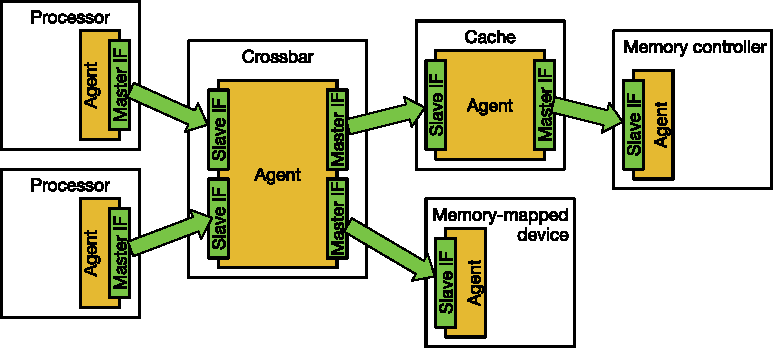
\includegraphics[width=0.8\textwidth]{TileLink_Topology.pdf}
    \caption{Connection model in \texttt{TileLink} and its interfaces. Source: \cite{sifive2018tilelink}}
    \label{fig:tilelink_connection_model}
\end{figure}

\texttt{TileLink} is a highly parameterizable, open-source, shared memory interconnect protocol based on the aforementioned crossbar structure, designed to connect diverse modules for SoCs. \texttt{TileLink} is implemented via a hierarchical, point-to-point network that can be easily scaled. This protocol provides memory-mapped access for multiple controllers, ensuring memory coherency while supporting efficient communication between processors, DMAs, and peripheral devices.

A \texttt{TileLink} bus system can support a combination of multiple communicating agents, each capable of supporting different configured subsets of the protocol. The \texttt{TileLink} specification includes three levels of operational configuration for agents, presented in Table \ref{tab:tilelink_configs}.

\begin{table}[h!]
\centering
\caption{\texttt{TileLink} operational configurations. Source: \cite{sifive2018tilelink}}
\label{tab:tilelink_configs}
\begin{tabular}{|l|c|c|c|}
\hline
 & \textbf{TL-UL} & \textbf{TL-UH} & \textbf{TL-C} \\
\hline
\textbf{Read/Write operations} & y & y & y \\
\textbf{Multibeat messages} & . & y & y \\
\textbf{Atomic operations} & . & y & y \\
\textbf{Hint operations} & . & y & y \\
\textbf{Cache block transfers} & . & . & y \\
\textbf{Channels B+C+E} & . & . & y \\
\hline
\end{tabular}
\end{table}

\texttt{TileLink} clearly distinguishes between cached and uncached communications. The simplest level is \texttt{TileLink} Uncached Lightweight (\texttt{TL-UL}), which only supports basic read and write operations to memory, for individual words. The next, more complex level is \texttt{TileLink} Uncached Heavyweight (\texttt{TL-UH}), which adds features such as "hints," "atomic" operations, and burst accesses but does not support coherent caching. Here, "hints" refers to a feature where a request command seeks data information external to the executing command from masters, and "atomic" refers to operations that lock access rights in a system with multiple masters, which could be microprocessors. Finally, \texttt{TileLink} Cached (\texttt{TL-C}) is the full protocol, supporting the use of coherent caches within the system.

For integrating peripheral hardware, all three bus configuration levels can be used. The communication connection diagram, at its most complete level, between a custom peripheral hardware and an agent is shown in Figure \ref{fig:tilelink_channels}.

\begin{figure}[h!]
    \centering
    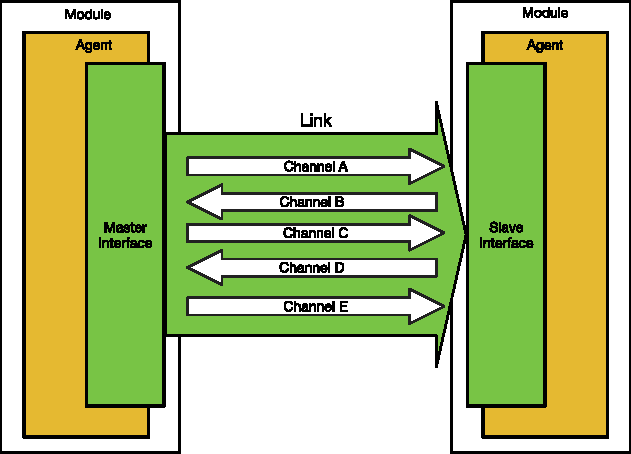
\includegraphics[width=0.8\textwidth]{TileLink_FiveChannel.pdf}
    \caption{Channels in a \texttt{TileLink} connection between two agents. Source: \cite{sifive2018tilelink}}
    \label{fig:tilelink_channels}
\end{figure}

In this \texttt{TileLink} protocol, the defined communication channels include \texttt{A}, \texttt{B}, \texttt{C}, \texttt{D}, and \texttt{E}, each undertaking specific roles in the interaction process between a master (M) and a slave (S), and all have a defined direction of transmission as depicted in the figure above.
\begin{itemize}
    \item \textbf{Channel A:} This is the initiation channel, where M sends requests to S, establishing the initial step of the communication process.
    \item \textbf{Channel B:} This channel is used when M requests a cache block from S, ensuring necessary data is queried.
    \item \textbf{Channel C:} Used for S to respond to M's request for a cache block, playing a crucial role in providing necessary data to M.
    \item \textbf{Channel D:} This is the general response channel, where S sends the final response to M after processing requests.
    \item \textbf{Channel E:} This channel ensures transaction completion by performing the final handshake for cache block transfer between the two parties.
\end{itemize}

The priority order for these channels is as follows: \texttt{A} < \texttt{B} < \texttt{C} < \texttt{D} < \texttt{E}, where channel \texttt{A} has the lowest priority and \texttt{E} has the highest. Prioritization in the \texttt{TileLink} bus system ensures that messages transmitted through the system do not fall into a hold-and-wait loop. In other words, the message flow through all channels between agents is maintained as a directed acyclic graph, enabling the \texttt{TileLink} protocol to operate without encountering deadlocks, ensuring continuous and uninterrupted data flow within the system.

% The choice of TileLink bus configuration depends on the component desired to be connected to the system; in this thesis, these are cryptographic algorithm accelerator cores designed separately using Verilog HDL. For this purpose, the TileLink configuration used for integration is TL-UL, which only includes channels A and D between M and S, as shown in Figure \ref{fig:tilelink_tl_ul_structure}.

The choice of \texttt{TileLink} bus configuration is relevant for connecting various memory-mapped peripherals within the system. For general-purpose MMIO peripherals, which might include cryptographic algorithm accelerators designed in \texttt{Verilog} HDL (if they were to be integrated as MMIO devices), the \texttt{TL-UL} configuration, comprising only channels \texttt{A} and \texttt{D} between M and S (as shown in Figure \ref{fig:tilelink_tl_ul_structure}), is often sufficient. However, for the primary accelerator in this thesis, the \texttt{Gemmini} core, integration is achieved through the \texttt{RoCC} interface, which provides a more tightly-coupled path to the processor core, rather than as a \texttt{TileLink}-attached MMIO peripheral. Details on the \texttt{RoCC} interface are discussed further in Section \ref{subsec:peripheral_components}. For other standard MMIO peripherals, a wrapper from the \texttt{Rocket Chip} library, using \texttt{Chisel}/\texttt{Scala}, can be inherited and customized to connect their signals to the appropriate system bus, typically the peripheral bus.


\begin{figure}[h!]
    \centering
    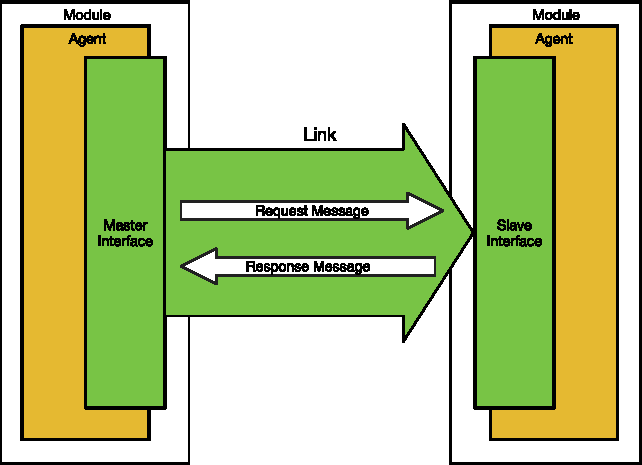
\includegraphics[width=0.7\textwidth]{TileLink_Overview.pdf} % Replace placeholder.png with your actual image file
    \caption{\texttt{TileLink} \texttt{TL-UL} connection structure. Source: \cite{sifive2018tilelink}}
    \label{fig:tilelink_tl_ul_structure}
\end{figure}

At the system configuration level, a wrapper from the \texttt{Rocket Chip} library, using \texttt{Chisel}/\texttt{Scala}, can be inherited and customized to convert the signals of the accelerator core to the system bus, in this case, the peripheral bus. Details for this interface will be further elaborated in subsequent sections of this thesis.

\subsection{Memory and Cache}
\label{subsec:memory_cache}

Each Tile in the system is integrated with a processor core and an L1 cache that is flexibly configurable. By default design with \texttt{Chisel}, the L1 cache has a size of 16 KiB, organized multi-dimensionally with sets and ways. The L1 cache uses a set-associative cache structure, dividing the memory region into sets, each set containing a fixed number of data blocks (ways). When a memory address access request occurs, the index derived from the address maps it to a specific set. The cache controller then searches for the data block within the ways of that set. This design supports both instruction and data storage, optimizing access performance and increasing the hit rate compared to caches with lower associativity.

In addition to the L1 cache, the system also integrates a shared L2 cache, connected to all cores via the \texttt{TileLink} bus system. The L2 cache acts as an intermediate storage repository, allowing processor cores and other components in the system to perform read/write data requests. This is a coordination mechanism that helps reduce pressure on the main memory and improves overall processing performance. The L2 cache controller also ensures fairness in resource allocation, using a queuing system to manage access requests.

At a higher level, the system also supports the integration of external memory, such as DRAM or SRAM, through open-source controllers or specialized IPs from FPGA implementation toolkits. Additionally, an interface with \texttt{DRAMSim} is supported for integration when performing full-system simulation. This provides flexibility and scalability, meeting various requirements in practical applications.

\subsection{Core-Complex}
\label{subsec:core_complex}

As previously mentioned, the \texttt{Chipyard} framework and library consist of many component definition classes that can form a \texttt{Rocket Chip} system. This allows for the formation of a complex system with diverse processor cores and peripherals, specifically heterogeneous architecture systems comprising multiple different processors like \texttt{Rocket} and \texttt{BOOM} coexisting on the system.

In these multi-core processor structures, each individual core will be uniquely identified with a different hart ID, ordered according to the system configuration. An example can be referenced below with a configuration comprising one \texttt{Rocket} core and one \texttt{BOOM} core. The corresponding block diagram configuration when generating the system will be as shown in Figure \ref{fig:heterogeneous_cores_system} below.

% Same, which one sounds better?
% As previously mentioned, the Chipyard framework and library consist of many component definition classes that can form a Rocket Chip system. This allows for the formation of a complex system with diverse processor cores and peripherals. A key capability is the creation of systems with heterogeneous architectures, potentially comprising multiple different processor cores like Rocket and BOOM coexisting on the same system, as illustrated in Figure \ref{fig:heterogeneous_cores_system}.

% In such multi-core processor structures, each individual processor core would be uniquely identified with a different hart ID, ordered according to the system configuration. For instance, a configuration might include one Rocket core alongside a BOOM core.

\begin{figure}[h!]
    \centering
    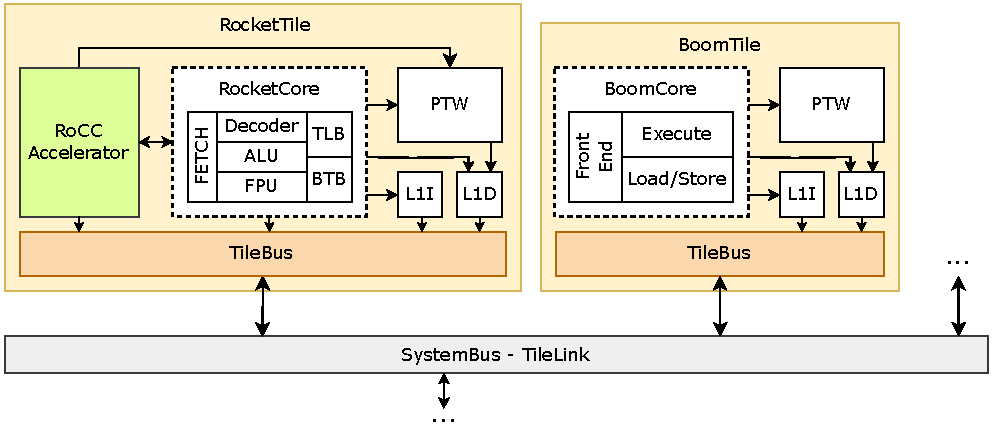
\includegraphics[width=0.8\textwidth]{RocketBOOM_CoreComplex.pdf} % Replace placeholder.png with your actual image file
    \caption{Implementation structure of a heterogeneous multi-core processor system.}
    \label{fig:heterogeneous_cores_system}
\end{figure}

A heterogeneous SoC system is an implementation approach also considered in this thesis to combine different processor cores to optimize performance and energy efficiency. At the application scale, lightweight cores can handle simple tasks with low power consumption, while high-performance cores support hyper-threading and out-of-order execution to process complex tasks. This design ensures flexibility, resource optimization, and superior performance for diverse applications.

\subsection{Peripheral Components}
\label{subsec:peripheral_components}

In the base system configuration class of \texttt{Rocket Chip}, many peripheral components are initialized and integrated by default to support both simulation and deployment on FPGA hardware for the SoC system. This configuration includes basic I/O devices such as PWM, interrupt controllers, JTAG, ROM, external memory, and standard peripheral interfaces, ensuring that basic communication, storage, and control requirements are met. In particular, common peripheral devices like UART, SPI Flash, and GPIO are implemented to support serial communication, storage management, and flexible control within the system.

\begin{figure}[h!]
    \centering
    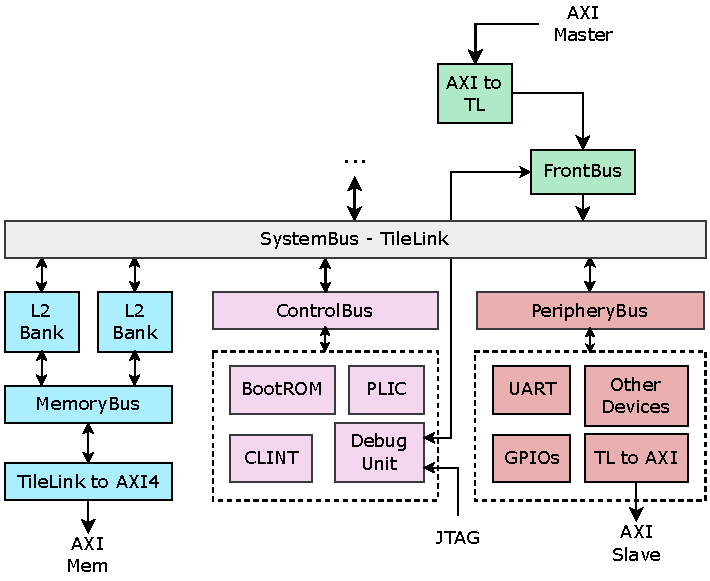
\includegraphics[width=0.8\textwidth]{RocketChip_Peripherals.pdf}
    \caption{Peripherals in the Rocket Chip base system.}
    \label{fig:rocketchip_base_peripherals}
\end{figure}

%  \begin{figure}[h!]
% \centering
% \includegraphics[width=0.8\textwidth]{placeholder.png} % Still using placeholder for this general example
% \caption{Implementation structure of a heterogeneous multi-core processor system (e.g., Rocket and BOOM). This illustrates a general capability of Chipyard.}
% \label{fig:heterogeneous_cores_system} % Kept the original label, adjust if needed
% \end{figure}

% A heterogeneous SoC with multiple distinct processor cores is an advanced implementation option that can be used to optimize performance and energy efficiency. At an application scale, lightweight cores could handle simple tasks with low power consumption, while high-performance cores could support features like hyper-threading and out-of-order execution for complex tasks. While the system developed in this thesis focuses on a single Rocket core augmented by the Gemmini RoCC accelerator, understanding Chipyard's capacity for heterogeneous multi-processor designs highlights its flexibility and potential for future, more complex applications. The design principles of modularity and clear interfacing within Chipyard facilitate such varied configurations.

All these components are developed based on the open-source \texttt{Rocket Chip} library, with hardware designs like \texttt{Rocket} and \texttt{BOOM} realized on the \texttt{Chisel} platform. When external memory is needed in design and simulation, the \texttt{AXI4} (Advanced eXtensible Interface 4) interface can be integrated as an intermediate layer, allowing effective connection with DRAM or SPI Flash models. Concurrently, serial protocols like JTAG are integrated to ensure accurate debugging capabilities and efficient serial communication, configured to connect with the \texttt{TileLink} bus. The \texttt{Rocket Chip} system also supports flexible configuration through special control ports, including custom boot pins and chip identification ports. Furthermore, the \texttt{Rocket Chip} system provides the capability to directly map bus interfaces such as \texttt{AXI4} Memory and MMIO (Memory-Mapped IO), allowing for expanded compatibility and optimized performance in complex SoC applications.

To expand the capability of integrating components and peripheral cores to form highly parameterized custom systems suitable for specific applications, the \texttt{Rocket Chip} architecture provides two flexible methods for peripheral integration. Specifically, the system can integrate a peripheral core as a \texttt{RoCC} (\texttt{Rocket} Custom Co-processor), located within each tile, or integrate at the system communication level via the MMIO mechanism. These methods facilitate in-depth customization, meeting various requirements for each specific application.

\begin{figure}[h!]
    \centering
    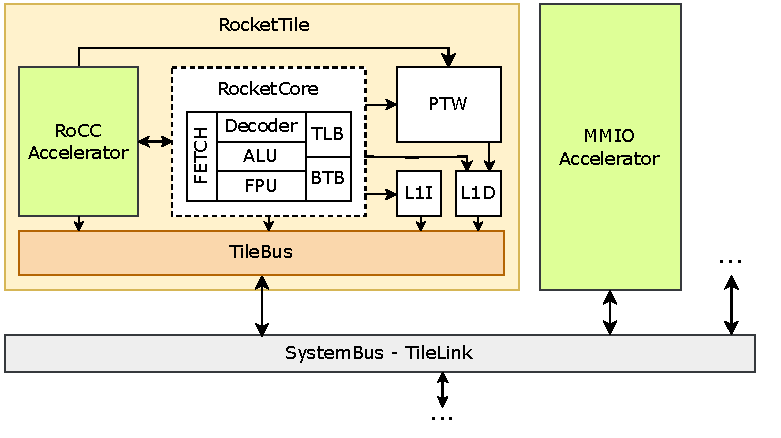
\includegraphics[width=0.8\textwidth]{RocketChip_WithMMIO.pdf} % Replace placeholder.png with your actual image file
    \caption{\texttt{RoCC} co-processor core and MMIO peripheral core in \texttt{Rocket Chip}.}
    \label{fig:rocc_mmio_rocketchip}
\end{figure}

MMIO Peripherals are custom peripherals attached directly to the \texttt{TileLink} bus, while Tightly-Coupled \texttt{RoCC} Accelerators are custom peripherals attached directly to the arbiter and processor within each Tile, in parallel with the processor core. With the \texttt{TileLink}-Attached MMIO method, the processor communicates with MMIO devices through registers mapped into memory at addresses on the system. Through these registers, control mechanisms or data transfer can be customized to suit the application of the peripheral core. Conversely, in the \texttt{RoCC} Accelerator method, communication is performed via a custom protocol and non-standard ISA instructions, which are configured and defined separately within the encoding space of the RISC-V ISA. For \texttt{Rocket} and \texttt{BOOM}, each core can control up to four accelerators through custom opcodes, sharing resources with the microprocessor. Instructions executed with \texttt{RoCC} cores have the format \texttt{customX rd, rs1, rs2, funct}. Here, \texttt{X} is a number from 0-3, determining the opcode that controls the routing of the instruction to a specific accelerator. The fields \texttt{rd}, \texttt{rs1}, \texttt{rs2} are the register numbers for the destination register and two source registers, and the \texttt{funct} field is a 7-bit integer that the accelerator can use to differentiate various instructions.

Peripherals connected as \texttt{RoCCs} have a distinct advantage due to their high customizability and direct connection and control via custom ISA instructions. This allows for specialized performance optimization, particularly useful for cores requiring large, complex computational workloads or applications needing extremely fast response times. Communication via a custom protocol and leveraging the RISC-V ISA helps \texttt{RoCC} utilize CPU resources efficiently, while also offering flexibility in designing specialized accelerator processors. The \texttt{Gemmini} accelerator, central to this thesis, is a prime example of a \texttt{RoCC}-based component, designed for high-throughput matrix multiplication and tightly integrated with the \texttt{Rocket} core.

While \texttt{RoCC} implementation can require a custom software toolchain for its specialized instructions, the performance benefits for demanding applications like those targeted by \texttt{Gemmini} often justify this investment. For this thesis, the integration of the \texttt{Gemmini} accelerator via the \texttt{RoCC} interface is deemed the most appropriate approach to achieve the desired performance for deep learning workloads.

Conversely, the MMIO \texttt{TileLink}-Attached method is widely used for integrating general-purpose memory-mapped peripheral devices. In this model, peripheral devices provide a set of registers (e.g., \texttt{Chisel} Registers) to communicate with microprocessors or other masters on the system bus. This method is suitable for peripherals where the tight coupling and custom instruction set of \texttt{RoCC} are not necessary.

To minimize design complexity for MMIO peripherals, the \texttt{Rocket Chip} architecture provides the \texttt{regmap} interface, which allows for the automatic generation of much of the necessary linking logic. Designers can use \texttt{TLRegisterRouter} or create a \texttt{LazyModule} and initialize \texttt{TLRegisterNode} to integrate such devices. Since \texttt{TileLink} is the official protocol used in SoCs based on \texttt{Rocket Chip} and \texttt{Chipyard}, designing MMIO peripheral devices (other than the primary \texttt{RoCC} accelerator) would typically focus on integration with this protocol.

% Original version
% However, this method also comes with some notable drawbacks. Firstly, implementing RoCC requires a custom software toolchain to synthesize special execution instructions, leading to longer development times and potentially increasing system complexity. Secondly, leveraging RoCC is only truly necessary for applications demanding extremely high performance; for use cases not requiring special optimization, this method may not provide value commensurate with the investment of effort. Dependence on non-standard instructions can reduce compatibility and scalability in diverse system designs. The development and integration of peripherals using the MMIO TileLink approach is deemed more suitable for the purposes of this thesis.

% The MMIO TileLink-Attached method is widely used in designing memory-mapped peripheral devices. In this model, peripheral devices provide a set of registers, specifically Chisel Registers, to communicate with microprocessors or other masters on the system bus. By writing data to these registers, microprocessors can adjust settings or send commands to the peripheral device or accelerator core. Conversely, by reading from these registers, the microprocessor can query the status or receive results and data from the peripheral device or accelerator core.

% To minimize design complexity, the Rocket Chip architecture provides the "regmap" interface, which allows for the automatic generation of much of the necessary linking logic. Instead of manually writing management nodes and register-exposing logic, designers can easily use TLRegisterRouter or create a LazyModule and initialize TLRegisterNode to integrate the device into the system. The simplest way to create an MMIO peripheral device is to use a configuration class like TLRegisterRouter, or AXI4RegisterRouter if choosing to use the AXI4 bus. This abstracts the details of the interconnect protocol with the peripheral bus (PBUS) and provides a convenient interface for defining memory-mapped registers. Since TileLink is the official protocol used in SoCs based on Rocket Chip and Chipyard, designing MMIO peripheral devices typically focuses on integration with this protocol, ensuring consistency and efficiency throughout the system.

% % !TeX root = main.tex
\chapter{Architectural Foundations of DNN Acceleration}
\label{ch:foundations}

% Chapter Introduction
The efficient execution of Deep Neural Networks (DNNs) presents one of the most significant challenges and opportunities in modern computer architecture. While today's general-purpose CPUs are highly optimized for a wide range of tasks, their fundamental design principles are often mismatched with the unique computational and data movement patterns of large-scale neural networks. This chapter will establish the foundational concepts that motivate the need for specialized hardware. We will begin by exploring the core problem---the immense cost of data movement---and then introduce the classic architectural paradigm designed to solve it: the systolic array. Finally, we will examine how this timeless principle is embodied in state-of-the-art industrial accelerators, providing the necessary context to understand the design of the Gemmini accelerator, which is the central subject of this thesis.

\section{The Data-Compute Divide: The Memory Wall}
\label{sec:memory_wall}

The performance of any computing system is ultimately limited by two factors: the speed of its computations and the speed at which it can supply data to its computational units. For decades, Moore's Law drove exponential growth in the number of transistors on a chip, leading to dramatic increases in processing power. However, the speed of off-chip memory systems, such as DRAM, has improved at a much slower pace. This growing disparity between processor speed and memory speed is famously known as the \textbf{Memory Wall} \cite{wulf1995hitting}.

For data-intensive workloads like DNNs, this is the primary performance bottleneck. The problem can be understood with a simple analogy: imagine a master chef (the processor) who can perform culinary tasks with superhuman speed. However, their ingredients (the data) are stored in a large warehouse across the street (DRAM). Even though the chef is exceptionally fast, their overall productivity is dominated by the time spent walking to and from the warehouse to fetch each ingredient.

This bottleneck is not just about latency; it is fundamentally about energy. As quantified by Horowitz \cite{horowitz2014energy}, the energy required to perform a complex 32-bit floating-point computation is dwarfed by the energy needed to fetch its operands from off-chip DRAM (Figure \ref{fig:energy_cost}). This immense energy cost of data movement means that for DNNs, which perform billions of operations, any viable high-performance hardware solution must be designed with a primary objective: to minimize data movement.

\begin{figure}[h!]
    \centering
    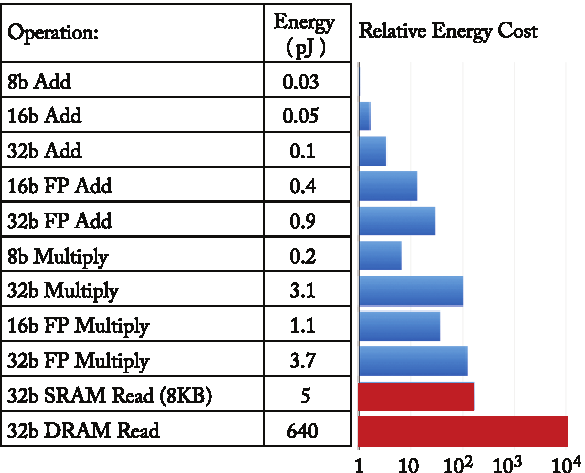
\includegraphics[width=0.8\textwidth]{EfficientDNN_EnergyConsumption.pdf} 
    \caption[The Relative Energy Cost of Computation vs. Memory Access]{The relative energy cost of various arithmetic and memory operations. A 32-bit DRAM read is orders of magnitude more costly than a 32-bit floating-point addition. This disparity is the primary motivation for specialized accelerator architectures. Adapted from Horowitz, as presented in Sze et al. \cite{sze2020efficient, horowitz2014energy}.}
    \label{fig:energy_cost}
\end{figure}

\section{A Classic Solution: The Systolic Principle}
\label{sec:systolic_principle}

In his seminal 1982 paper, H.T. Kung proposed a novel architectural paradigm designed specifically to address the memory wall: the \textbf{systolic array} \cite{kung1982systolic}. The architecture is named by analogy to the human circulatory system. Just as the heart rhythmically pumps blood to the body's cells, in a systolic system, memory "pumps" data through a regular grid of simple Processing Elements (PEs).

The core principle is to \textbf{maximize the number of computations performed for each data item fetched from memory}. Instead of fetching an operand, using it once in a central ALU, and then discarding it (the conventional approach), a systolic array passes an operand from one PE to the next in a pipelined fashion. At each step of its journey, the data element participates in another computation. This structure, illustrated conceptually in Figure \ref{fig:conventional_vs_systolic}, amortizes the high cost of the initial memory access over dozens or even hundreds of useful operations.

\begin{figure}[htbp]
    \centering
    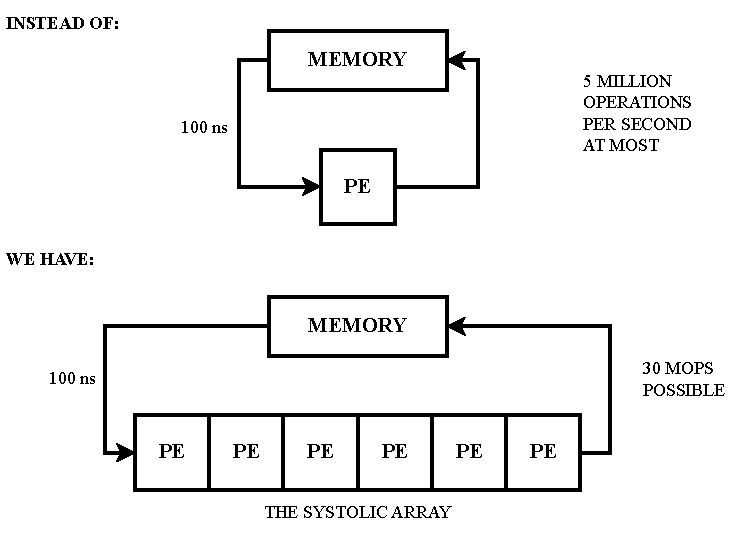
\includegraphics[width=0.9\textwidth]{SystolicArray_Kung1982.pdf} 
    \caption[Conventional vs. Systolic Processing]{A conceptual comparison of a conventional von Neumann architecture and a systolic architecture. The conventional approach (top) is bottlenecked by the memory bus. The systolic approach (bottom) uses an array of PEs to achieve high throughput with the same memory bandwidth by reusing data internally. Adapted from the presentation of Kung's work \cite{kung1982systolic}.}
    \label{fig:conventional_vs_systolic}
\end{figure}

\section{Case Studies in Modern Systolic Design}
\label{sec:case_studies}
While the systolic principle is four decades old, it has become the dominant paradigm for modern high-performance DNN accelerators. We will examine two landmark industrial designs that showcase this principle in practice.

\subsection{Google's TPUv1: A Datacenter-Scale Design}
Google's Tensor Processing Unit (TPU) was one of the first large-scale custom ASICs designed specifically for accelerating DNN inference in datacenters \cite{jouppi2017tpu}. As shown in Figure \ref{fig:tpu_diagram}, its architecture is a direct embodiment of the systolic principle. The heart of the TPU is a massive 256x256 Matrix Multiply Unit, which is a two-dimensional systolic array of 65,536 8-bit multiply-accumulate (MAC) units. To feed this vast computational engine, the TPU relies on a large, software-controlled on-chip memory called the Unified Buffer (a 24 MiB scratchpad), which stores input activations and intermediate partial sums. The design philosophy of the TPU prioritizes deterministic, high-throughput performance for inference tasks where low latency is critical.

\begin{figure}[h!]
    \centering
    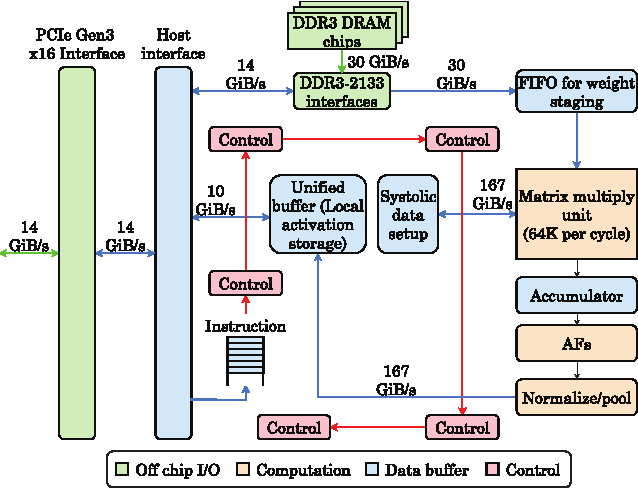
\includegraphics[width=0.9\textwidth]{TPU_v1_Overview.pdf} 
    \caption[The Google TPUv1 Block Diagram]{A high-level block diagram of the Google TPUv1. The design is dominated by the systolic Matrix Multiply Unit and its large on-chip Unified Buffer. Adapted from Jouppi et al. \cite{jouppi2017tpu, mittal2021survey}.}
    \label{fig:tpu_diagram}
\end{figure}

\subsection{NVIDIA NVDLA: An Open-Source Accelerator IP}
In contrast to the monolithic, datacenter-focused TPU, the NVIDIA Deep Learning Accelerator (NVDLA) is an open-source, configurable IP core designed for integration into a wide range of Systems-on-Chip (SoCs), particularly for embedded systems \cite{farshchi2019nvdla}. As shown in Figure \ref{fig:nvdla_diagram}, the NVDLA has a more modular design, with a dedicated Convolutional Core (which contains the MAC units), a Post-Processing unit for activation functions and pooling, and a Convolutional Buffer for storing weights and inputs. Unlike the TPU's custom interface, the NVDLA uses industry-standard bus protocols (AXI and APB) for memory access and control, simplifying its integration into third-party SoC designs. Its configurability (e.g., \texttt{nv\_small}, \texttt{nv\_large}) allows a system designer to trade off area and performance, making it a flexible solution for the embedded space.

\begin{figure}[htbp]
    \centering
    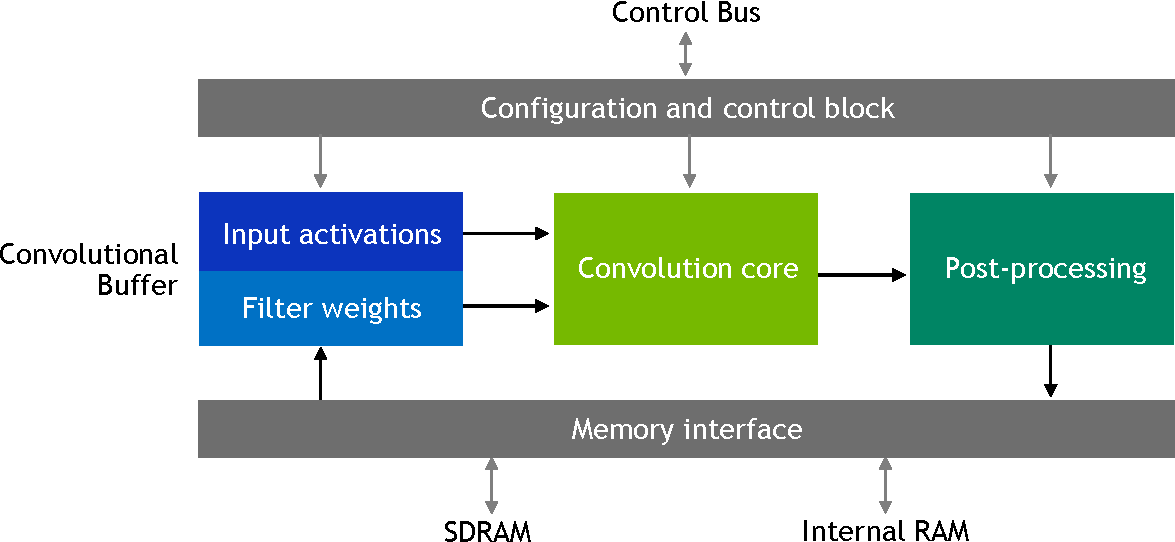
\includegraphics[width=\textwidth]{NVDLA_ArchitectureOverview.pdf} 
    \caption[The NVDLA High-Level Architecture]{The high-level architecture of the NVDLA. The design is partitioned into distinct functional units connected via standard bus interfaces. Adapted from Farshchi et al. \cite{farshchi2019nvdla}.}
    \label{fig:nvdla_diagram}
\end{figure}

\section{A Formal Framework: Dataflows}
\label{sec:formal_dataflows}
The design choices made in architectures like the TPU and NVDLA can be formally described using the concept of a \textbf{dataflow}. The dataflow defines the strategy for moving data through the systolic array to maximize reuse. The effectiveness of a given dataflow depends on the structure of the DNN layer being executed. The two most common dataflows, which we will see are directly relevant to Gemmini, are:
\begin{itemize}
    \item \textbf{Weight Stationary (WS):} This dataflow prioritizes weight reuse. Filter weights are pre-loaded into the PEs and remain stationary, while input activations are streamed in. This strategy, used by the Google TPU, is highly efficient for layers with large input feature maps and relatively small filters.
    \item \textbf{Output Stationary (OS):} This dataflow prioritizes minimizing the movement of partial sums. Each PE is responsible for accumulating the final value for a single output activation, which remains stationary in its accumulator. Inputs and weights are streamed to the PE as needed. This can be more efficient for layers where partial sum read/write energy is a dominant cost.
\end{itemize}
These strategies, visually contrasted in Figure \ref{fig:dataflow_taxonomy} and \ref{fig:dataflow_comparison}, represent a fundamental trade-off in accelerator design. The choice of dataflow directly impacts which types of data reuse, shown in Figure \ref{fig:dnn_reuse}, are most effectively exploited.

\begin{figure}[htbp]
    \centering
    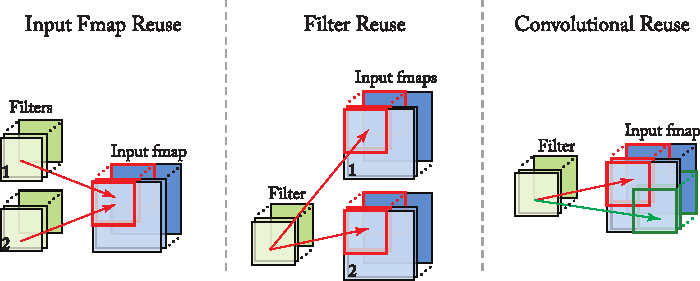
\includegraphics[width=0.9\textwidth]{EfficientDNN_DataReuse.pdf} 
    \caption[Data Reuse Opportunities in DNNs]{The three primary forms of data reuse in convolutional layers: convolutional, filter, and input reuse. Adapted from Sze et al. \cite{sze2020efficient}.}
    \label{fig:dnn_reuse}
\end{figure}

\begin{figure}[htbp]
    \centering
    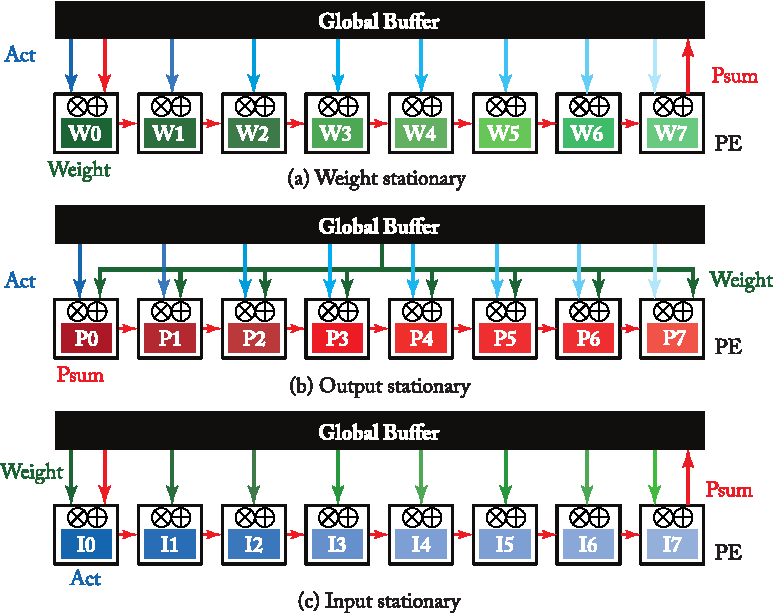
\includegraphics[width=0.9\textwidth]{EfficientDNN_ModernDataflow.pdf} 
    \caption[Taxonomy of Common DNN Dataflows]{A visual comparison of Weight Stationary (left) and Output Stationary (right) dataflows. Adapted from Sze et al. \cite{sze2020efficient}.}
    \label{fig:dataflow_taxonomy}
\end{figure}

\begin{figure}[htbp]
    \centering
    \begin{subfigure}[b]{0.48\textwidth}
        \centering
        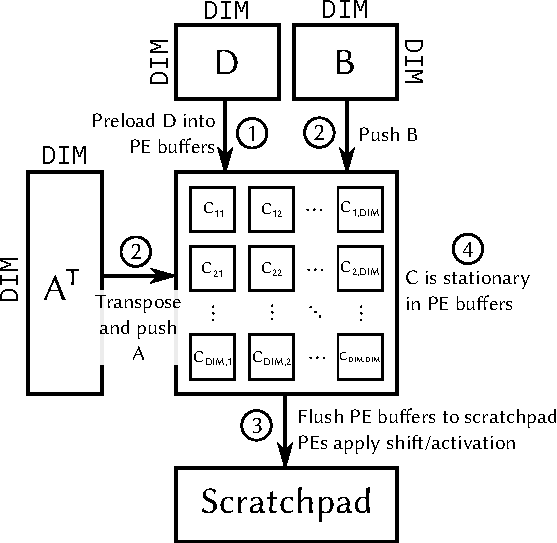
\includegraphics[width=\textwidth]{Gemmini_compute_os.pdf}
        \caption{Output Stationary (OS)}
        \label{fig:os_dataflow}
    \end{subfigure}
    \hfill
    \begin{subfigure}[b]{0.48\textwidth}
        \centering
        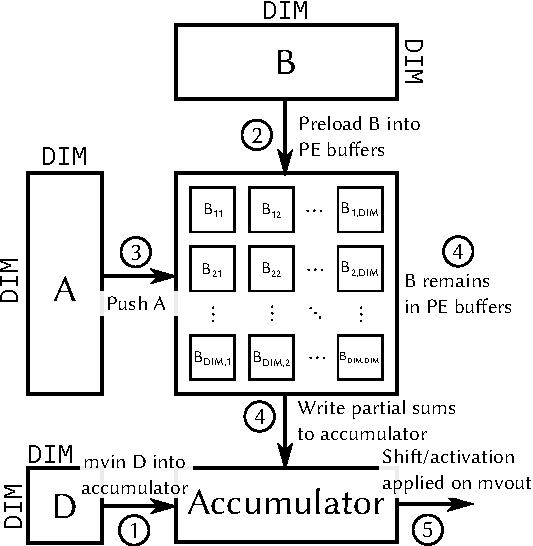
\includegraphics[width=\textwidth]{Gemmini_compute_ws.pdf}
        \caption{Weight Stationary (WS)}
        \label{fig:ws_dataflow}
    \end{subfigure}
    \caption[Comparison of OS and WS Dataflows]{A visual comparison of the two primary dataflows supported by Gemmini. (a) In the \textbf{Output Stationary} dataflow, the result matrix C remains stationary in the PEs to accumulate partial sums. (b) In the \textbf{Weight Stationary} dataflow, the weight matrix B is preloaded and remains stationary in the PEs to maximize weight reuse. The choice between these strategies represents a fundamental trade-off in accelerator design. Source: \cite{gemini-dac}.}
    \label{fig:dataflow_comparison}
\end{figure}

\section{Chapter Summary}
This chapter has built a foundational argument for the necessity of specialized hardware for DNN acceleration. We began with the core architectural challenge, the Memory Wall, and introduced the systolic array as a classic and enduring solution that minimizes costly data movement by maximizing data reuse. By examining modern industrial accelerators like the Google TPU and NVDLA, we have seen this principle in action. Finally, we formalized these strategies with the concept of dataflows, such as Weight Stationary and Output Stationary. These foundational concepts provide the necessary framework to understand the design and operation of the Gemmini accelerator, which will be the focus of the subsequent chapters.

% % !TeX root = main.tex
\chapter{The Gemmini DNN Accelerator: An Architectural Overview}
\label{chap:gemmini_overview}

As established in the previous chapter, the System-on-Chip (SoC) developed in this thesis utilizes a single \texttt{Rocket} Core augmented with a specialized accelerator for deep learning workloads. This chapter delves into the architecture of this accelerator: \texttt{Gemmini}, a sophisticated component designed to overcome the fundamental limitations of general-purpose processors for Deep Neural Network (DNN) tasks.

\begin{figure}[htbp]
    \centering
    
\includegraphics[width=0.9\textwidth]{Gemmini_Logo.pdf}
    \caption{Gemmini Logo. Source: \cite{gemini-dac}.}
    \label{fig:gemmini_logo}
\end{figure}

\section{Introduction: The Full-Stack Accelerator Philosophy}
\label{sec:gemmini_intro}

\texttt{Gemmini} is an open-source, full-stack DNN accelerator \textit{generator} developed at the University of California, Berkeley \cite{gemini-dac}. It is designed not merely as a standalone hardware component, but as a complete ecosystem for exploring and evaluating domain-specific hardware acceleration. 

Its design is rooted in the philosophy of "full-stack" evaluation. Many accelerators are designed and tested in isolation, which fails to account for critical system-level effects such as memory bus contention, cache coherency overhead, and operating system interactions (e.g., page faults and context switches) \cite{gemini-dac}. By generating not only the accelerator RTL but also a complete, Linux-capable SoC using the \texttt{Chipyard} framework, \texttt{Gemmini} enables a comprehensive analysis of these cross-stack interactions. This allows for a more realistic assessment of real-world performance and energy efficiency \cite{gemini-dac}.

Crucially, as a generator written in Chisel, \texttt{Gemmini} is not a single, fixed hardware design. As illustrated in Figure \ref{fig:gemmini_flexibility}, its flexible template can be configured to produce a wide spectrum of systolic architectures, from highly pipelined designs to parallel-vector engines. This makes it an exceptionally powerful platform for the academic exploration of accelerator architectures.

For this thesis, leveraging Gemmini provides the opportunity to explore a powerful DNN accelerator within a realistic SoC environment.

\begin{figure}[h!]
    \centering
    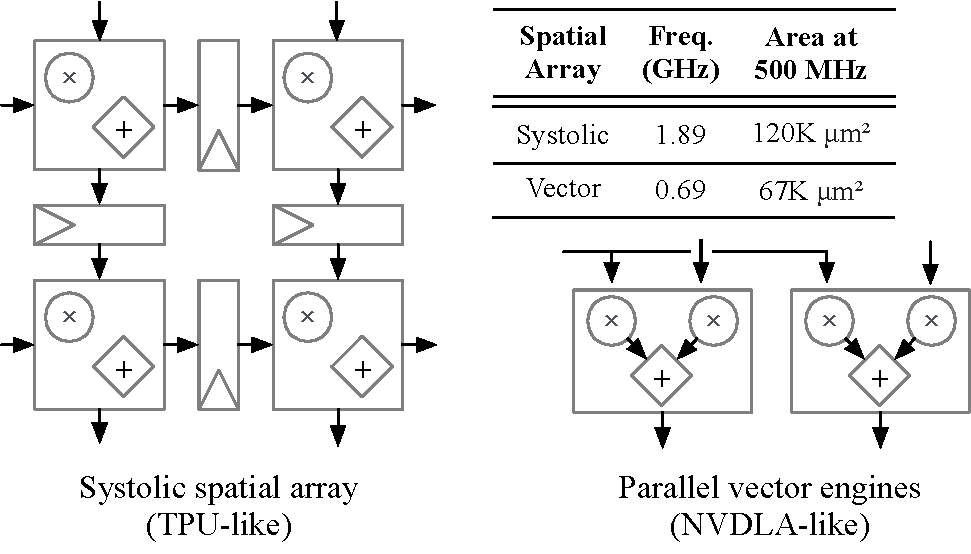
\includegraphics[width=0.9\textwidth]{Gemmini_SystolicNVDLA.pdf} 
    \caption[Architectural Flexibility of the Gemmini Generator]{The design space enabled by the Gemmini generator, allowing it to produce a wide variety of spatial array structures. Source: \cite{gemini-dac}.}
    \label{fig:gemmini_flexibility}
\end{figure}

\section{Top-Level Architectural Blueprint}
\label{sec:gemmini_blueprint}
The Gemmini generator can produce a wide range of accelerator instances based on a flexible architectural template. To understand the Gemmini architecture, we first examine the high-level template shown in Figure \ref{fig:gemmini_template}. This blueprint illustrates the three primary components of the accelerator---the Controller, the on-chip memory (Scratchpad and Accumulator), and the compute core (Spatial Array)---and their interface with the host CPU and system DRAM. The following sections provide a detailed analysis of each of these blocks.

\begin{figure}[htbp]
    \centering
    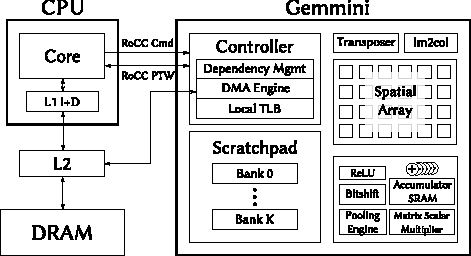
\includegraphics[width=0.9\textwidth]{Gemmini_ArchitectureOverview.pdf}
    \caption{High-level overview of the Gemmini accelerator template integrated with a host CPU and system memory hierarchy. Source: \cite{gemini-dac}.}
    \label{fig:gemmini_template}
\end{figure}

\section{Analysis of Core Architectural Components}
\label{sec:gemmini_components}

\subsection{The Systolic Compute Engine}
The computational heart of Gemmini is its systolic array, a highly configurable spatial array that functions as a powerful General Matrix-Matrix Multiplication (GEMM) engine. The array's microarchitecture, as detailed in Figure \ref{fig:gemmini_microarch}, features a two-level hierarchy composed of Tiles and individual Processing Elements (PEs). Each PE is capable of performing a Multiply-Accumulate (MAC) operation in a single clock cycle. This hierarchical and configurable design allows Gemmini to efficiently execute the dense matrix multiplications fundamental to modern Deep Neural Networks (DNNs).

\begin{figure}[htbp]
    \centering
    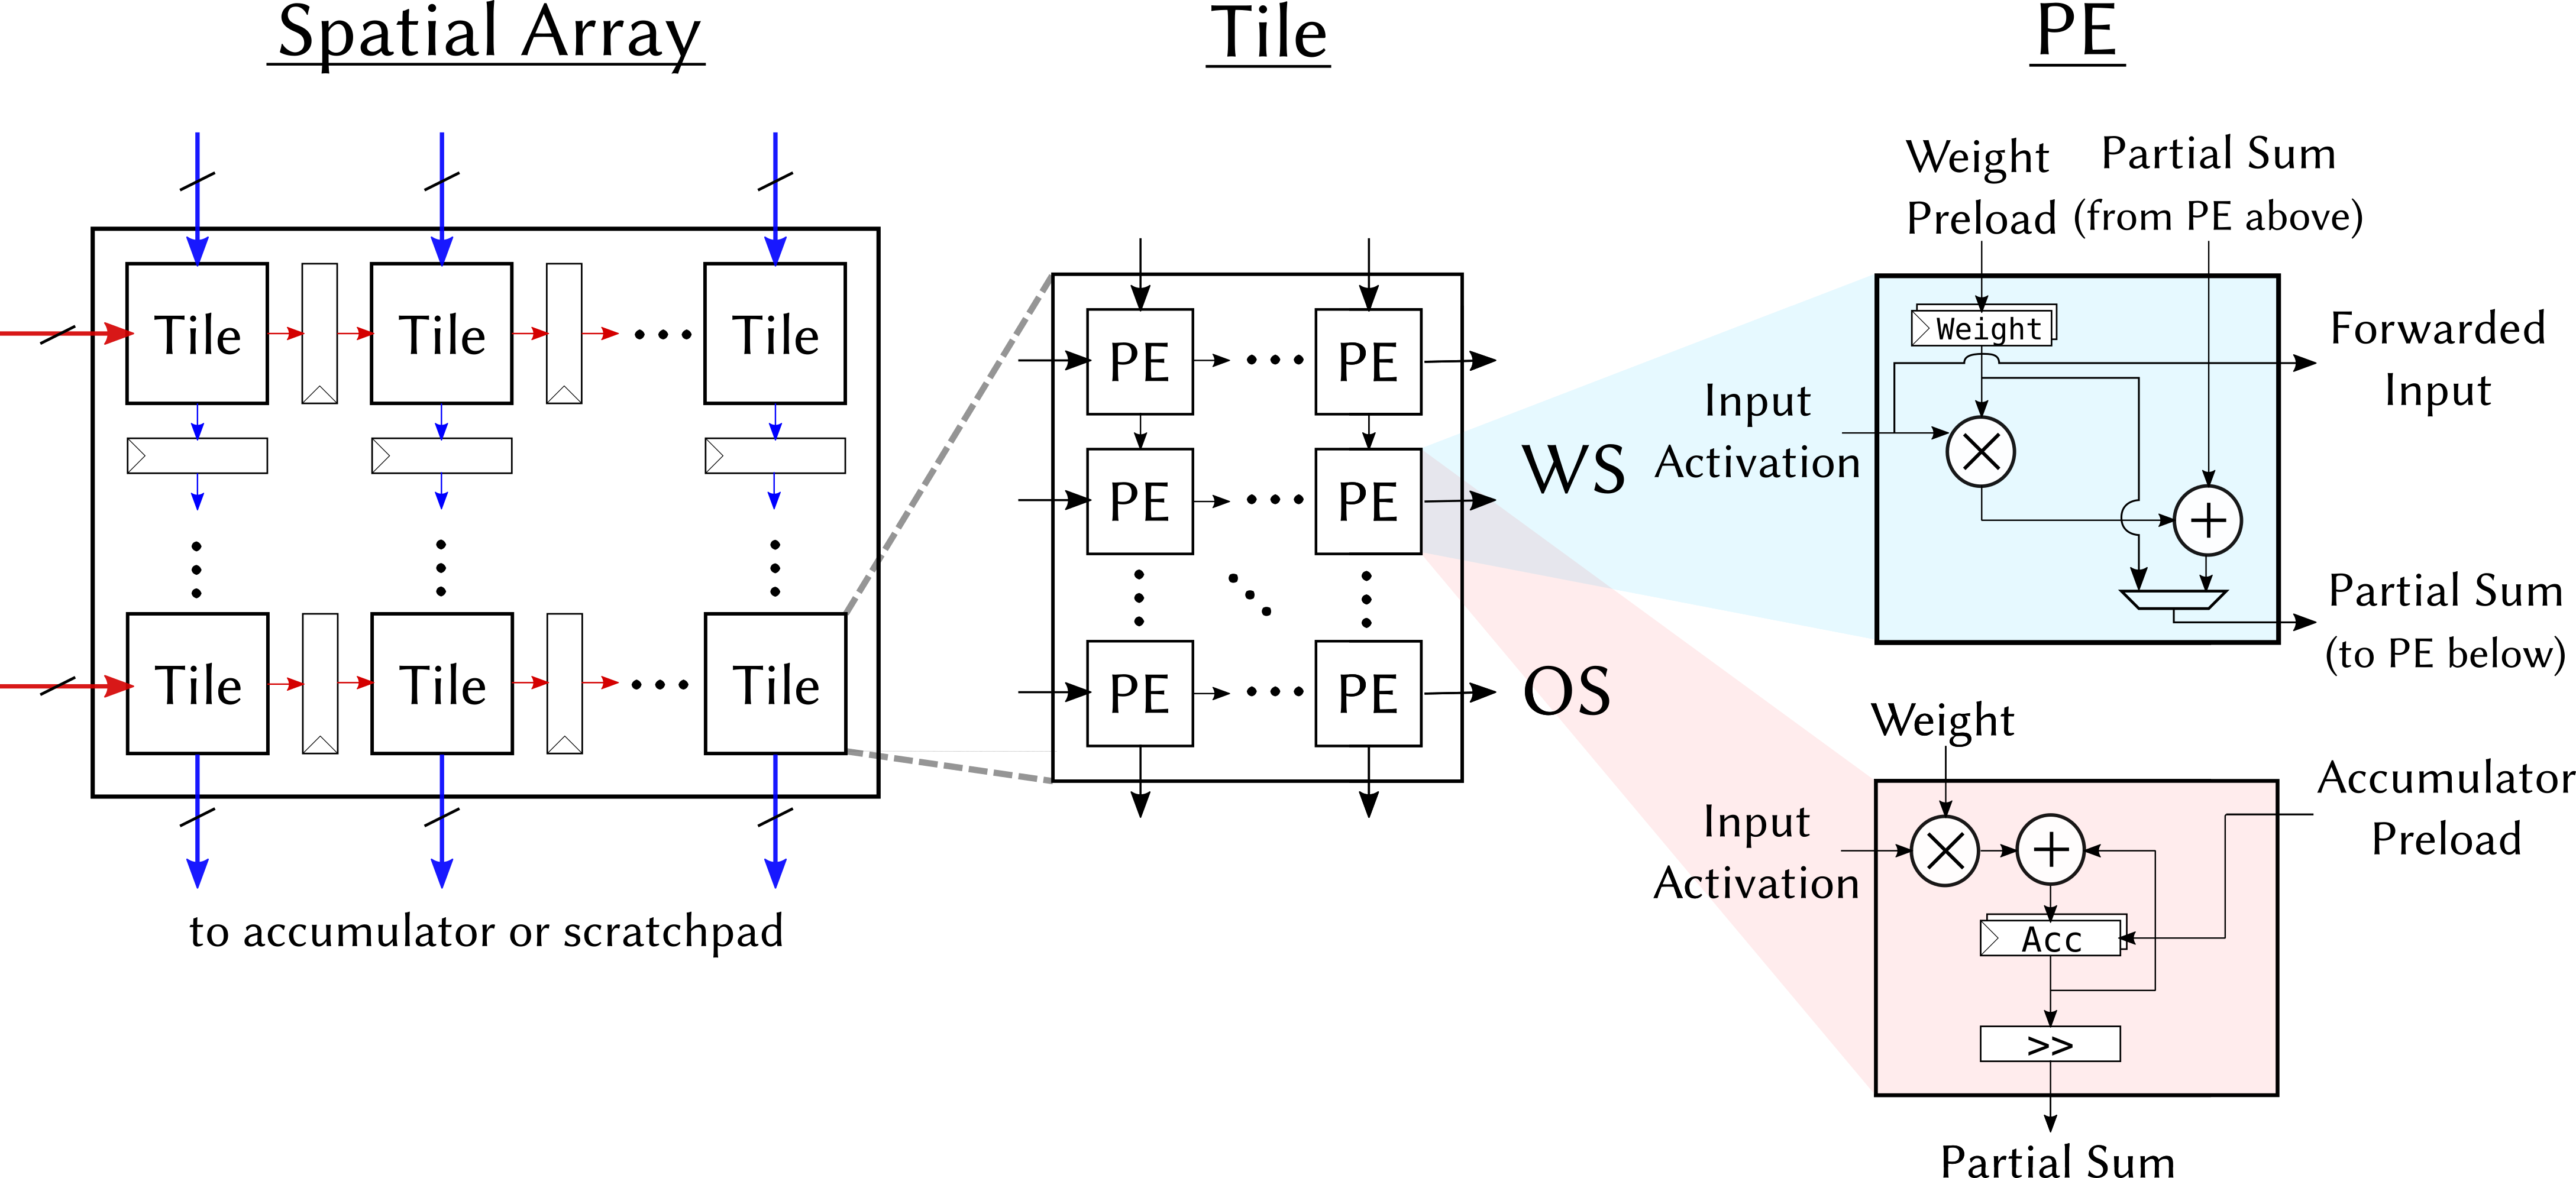
\includegraphics[width=\textwidth]{Gemmini_MicroArchitecture.png}
    \caption[Microarchitecture of Gemmini's Spatial Array]{The two-level hierarchy of Gemmini's spatial array, composed of tiles and Processing Elements (PEs). Source: \cite{gemini-dac}.}
    \label{fig:gemmini_microarch}
\end{figure}

The key parameters of the systolic array can be specified at generation time:
\begin{itemize}
    \item \textbf{Dimensions:} The size of the PE grid, structured into a hierarchy of tiles, can be configured (e.g., a 16x16 array composed of 2x2 tiles, each with 8x8 PEs). This allows for a trade-off between hardware area and parallel processing capability.
    \item \textbf{Dataflow:} Gemmini primarily supports two dataflow strategies: Weight Stationary (WS) and Output Stationary (OS). 
    \begin{itemize}
        \item In \textbf{WS dataflow}, the DNN weights are pre-loaded into the PEs and remain stationary, maximizing weight reuse as input activations are streamed through. 
        \item In \textbf{OS dataflow}, partial sums of the output activations remain stationary within the PEs, while both inputs and weights are streamed. This is particularly beneficial for layers with low weight reuse.
    \end{itemize}
    The choice of dataflow has a significant impact on performance and energy efficiency.
    \item \textbf{Pipelining:} The degree of pipelining within the array and its PEs can be configured, affecting the maximum clock frequency and overall throughput.
\end{itemize}

\subsubsection{Mapping Convolution to Hardware: The \texttt{im2col} Transformation}
\label{subsubsec:im2col}
While systolic arrays are fundamentally designed to accelerate General Matrix-Matrix Multiplication (GEMM), they are adept at accelerating 2D convolutions through a crucial data-restructuring technique known as \texttt{im2col} ("image-to-column"). This process unrolls the overlapping input image patches from a convolutional layer into the columns of a new, larger matrix. As shown in Figure \ref{fig:im2col}, this new matrix can then be multiplied with a corresponding weight matrix, effectively \textbf{converting the convolution into a GEMM operation} that the systolic array can process with maximum efficiency.

Recognizing the computational cost of this pre-processing step, Gemmini can be configured with a dedicated hardware unit to perform the \texttt{im2col} transformation on-the-fly. This offloads the data restructuring from the host CPU, freeing it for other tasks and streamlining the overall computation pipeline. The decision to include this unit represents a classic area-versus-performance trade-off in the accelerator design.

\begin{figure}[h!]
    \centering
    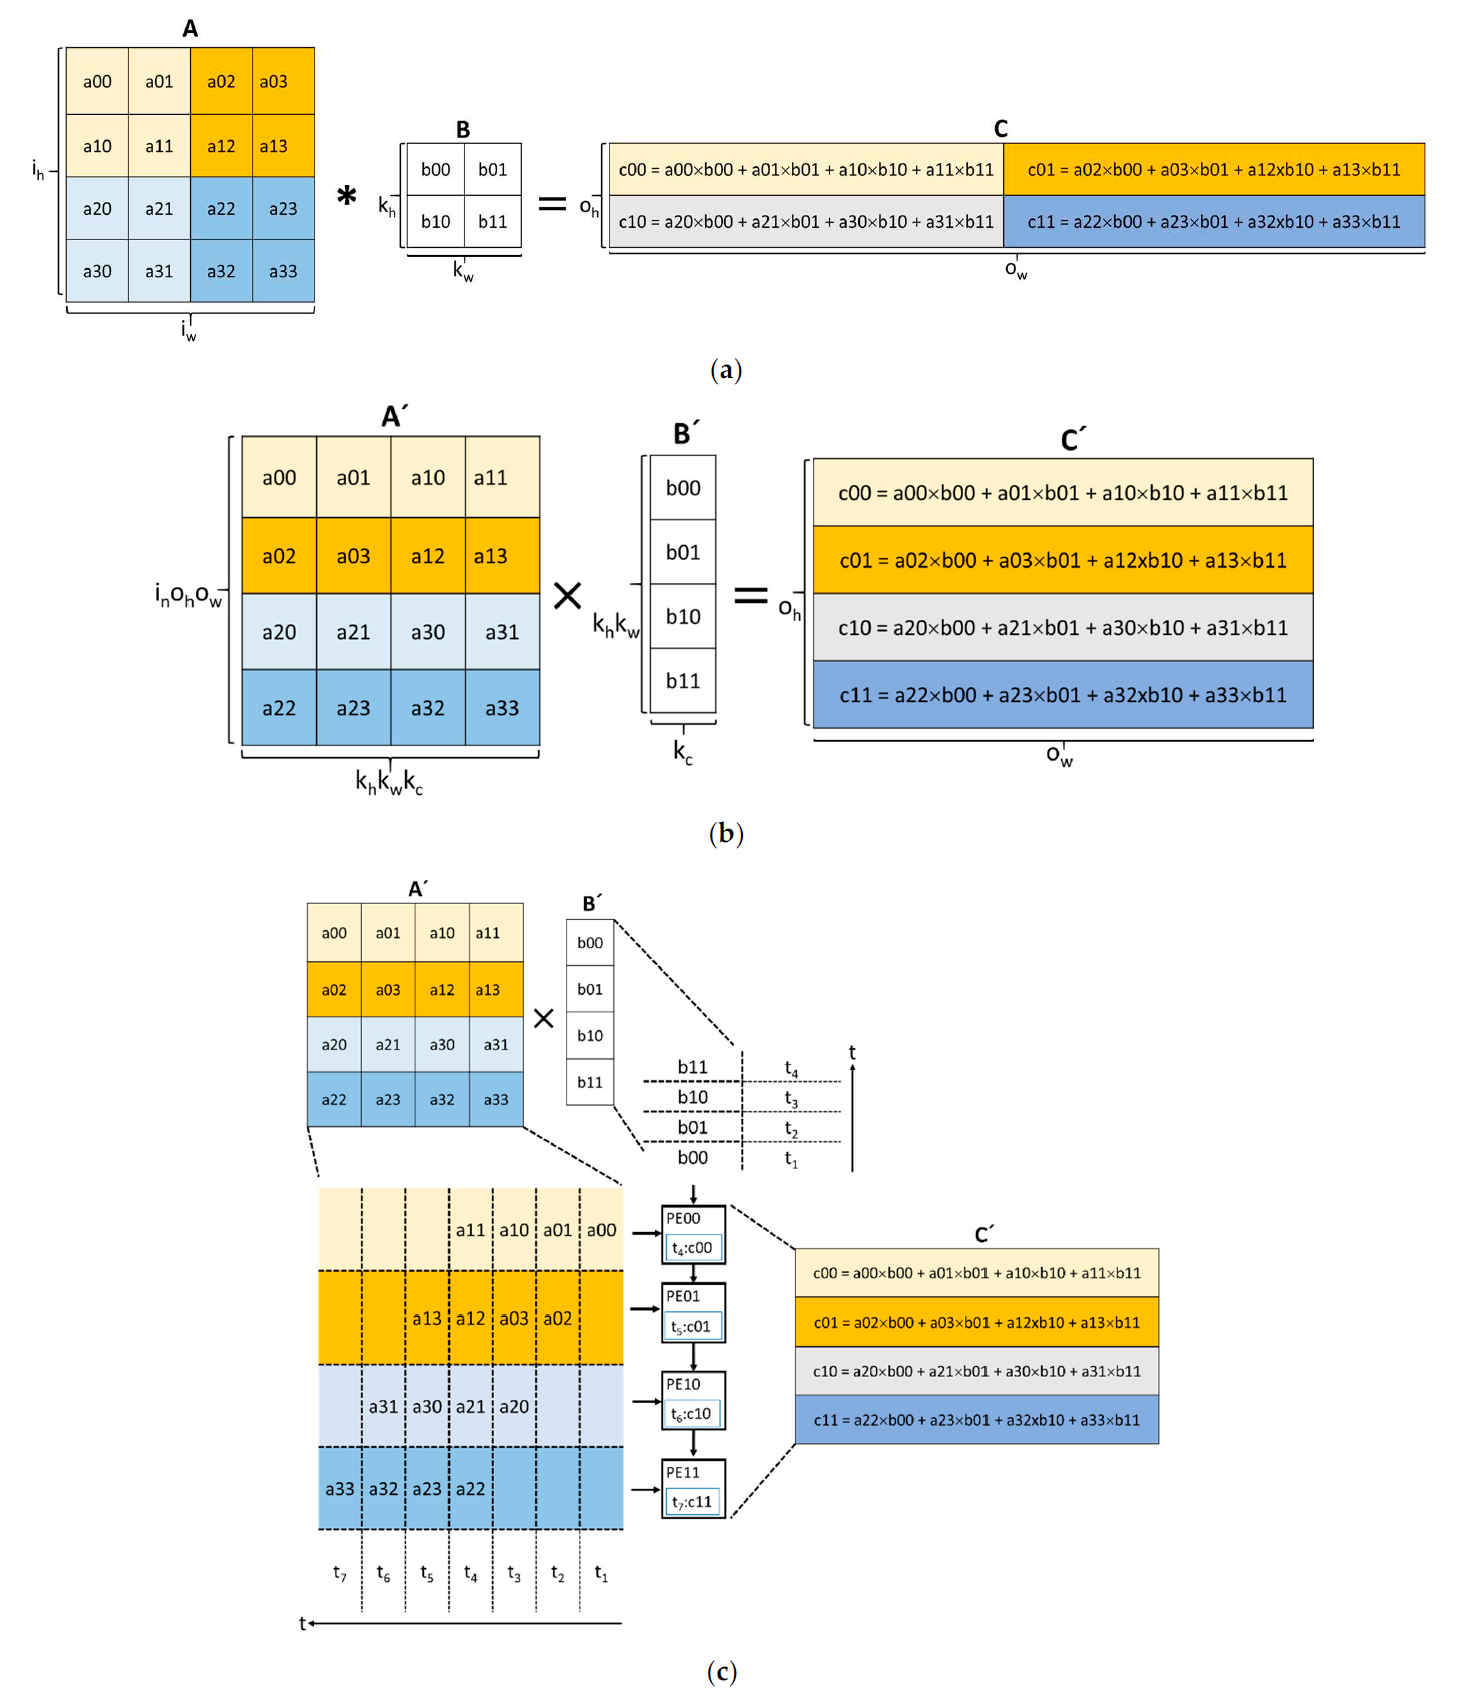
\includegraphics[width=\textwidth]{Gemmini_Im2Col.png}
    \caption[The im2col Transformation]{From convolution to systolic array computation: (a) direct convolution operation; (c) example of a systolic array operation; (b) A visualization of the \texttt{im2col}-based GEMM operation. The 3D input tensor (left) is transformed into a 2D matrix (center) that can be processed by the systolic array. Adapted from Gookyi et al. \cite{gookyi2023gemmini_case_study}.}
    \label{fig:im2col}
\end{figure}


\subsection{The On-Chip Memory Subsystem}
To feed its high-throughput systolic array, Gemmini includes a specialized on-chip memory system. This design represents a deliberate trade-off between hardware-managed caches and software-managed memories.
\begin{itemize}
    \item \textbf{Scratchpad Memory:} A software-managed SRAM used for staging input activations, weights, and intermediate feature maps close to the systolic array. Its purpose is to reduce the latency and energy consumption associated with fetching data from higher levels of the memory hierarchy, such as the shared L2 cache or main memory (DRAM). Its capacity and banking are configurable.
    \item \textbf{Accumulator Memory:} Separate from the main scratchpad, Gemmini features a dedicated memory to store the partial sums generated by the MAC operations. This memory typically uses a higher precision data type (e.g., 32-bit integers) than the input data (e.g., 8-bit integers) to maintain accuracy during accumulation.
\end{itemize}

\section{SoC Integration and System-Level Features}
\label{sec:gemmini_integration}

\subsection{The RoCC Coprocessor Interface}
Gemmini integrates into the Chipyard SoC via the \textbf{Rocket Custom Coprocessor (RoCC)} interface. As a tightly-coupled coprocessor, it receives custom RISC-V instructions dispatched directly by the host Rocket Core's pipeline. This allows for low-latency command and control.



This integration uses a decoupled access-execute model, as illustrated conceptually in Figure~\ref{fig:decoupled_pipelines}. The host CPU issues three main types of commands to Gemmini: load (from main memory to scratchpad), execute (perform computation on data within the scratchpad), and store (from scratchpad to main memory). These commands are placed into separate hardware queues, allowing Gemmini's internal controller then processes these commands asynchronously, and Gemmini's DMA engine to handle data movement in parallel with the systolic array's computations. This overlapping of communication and computation is crucial for hiding memory latency and maximizing the utilization of the systolic array.

\begin{figure}[htbp]
    \centering
    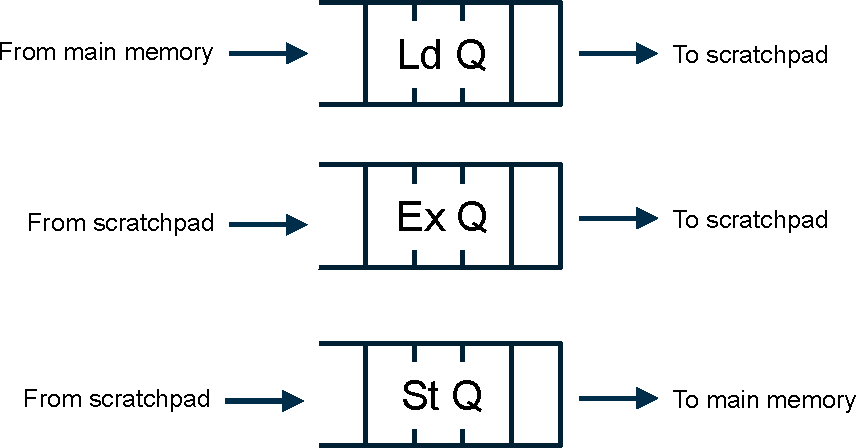
\includegraphics[width=0.8\textwidth]{Gemmini_DecoupledAccessExecutePipeline.pdf}
    \caption{Conceptual view of Gemmini's decoupled access-execute pipelines, managed by separate hardware command queues for Load, Execute, and Store operations. Source: \cite{gemini-dac}.}
    \label{fig:decoupled_pipelines}
\end{figure}

\subsection{Virtual Memory Support}
To operate correctly under a full-featured operating system like Linux, an accelerator's DMA engine must be able to translate virtual memory addresses into physical addresses. Gemmini is designed with this "full-stack" capability. It can be configured to share the host CPU's Page Table Walker (PTW) to perform its own address translations, and it includes its own local Translation Lookaside Buffer (TLB) to cache these translations and reduce latency.

\section{Summary}
\label{sec:gemmini_overview_summary}
In summary, Gemmini is a sophisticated, highly configurable DNN accelerator generator that embodies the principles of systolic computation. Its key architectural features include a powerful systolic array, a specialized on-chip memory hierarchy, and a tightly-coupled integration with a host processor via the \texttt{RoCC} interface, including support for system-level features like virtual memory. This design enables the high-performance execution of DNN workloads within a full-stack, system-level context. 

Having established this architectural overview, the following chapter will now perform a deep dive into the specifics of Gemmini's internal command processing and its multi-level programming model.

% % !TeX root = main.tex
\chapter{Gemmini's Internal Architecture and Programming Model}
\label{chap:gemmini_internals}

While Chapter \ref{chap:gemmini_overview} described the conceptual architecture of Gemmini, this chapter explores its internal structure and the software interfaces used to control it. A deeper understanding of these implementation-level details is necessary to effectively program the accelerator and analyze its performance.

\section{Internal Command and Control Flow}
\label{sec:gemmini_internal_flow}

A custom \texttt{RoCC} instruction sent from the Rocket core is not executed directly by the systolic array. Instead, it triggers a complex sequence of events within the Gemmini accelerator's internal controller modules. The overall structure of the generated hardware, as analyzed by Gookyi et al. \cite{gookyi2023gemmini_case_study}, is shown in Figure~\ref{fig:gemmini_internal_modules}. This section details the key components of this internal pipeline.

\begin{figure}[htbp]
    \centering
    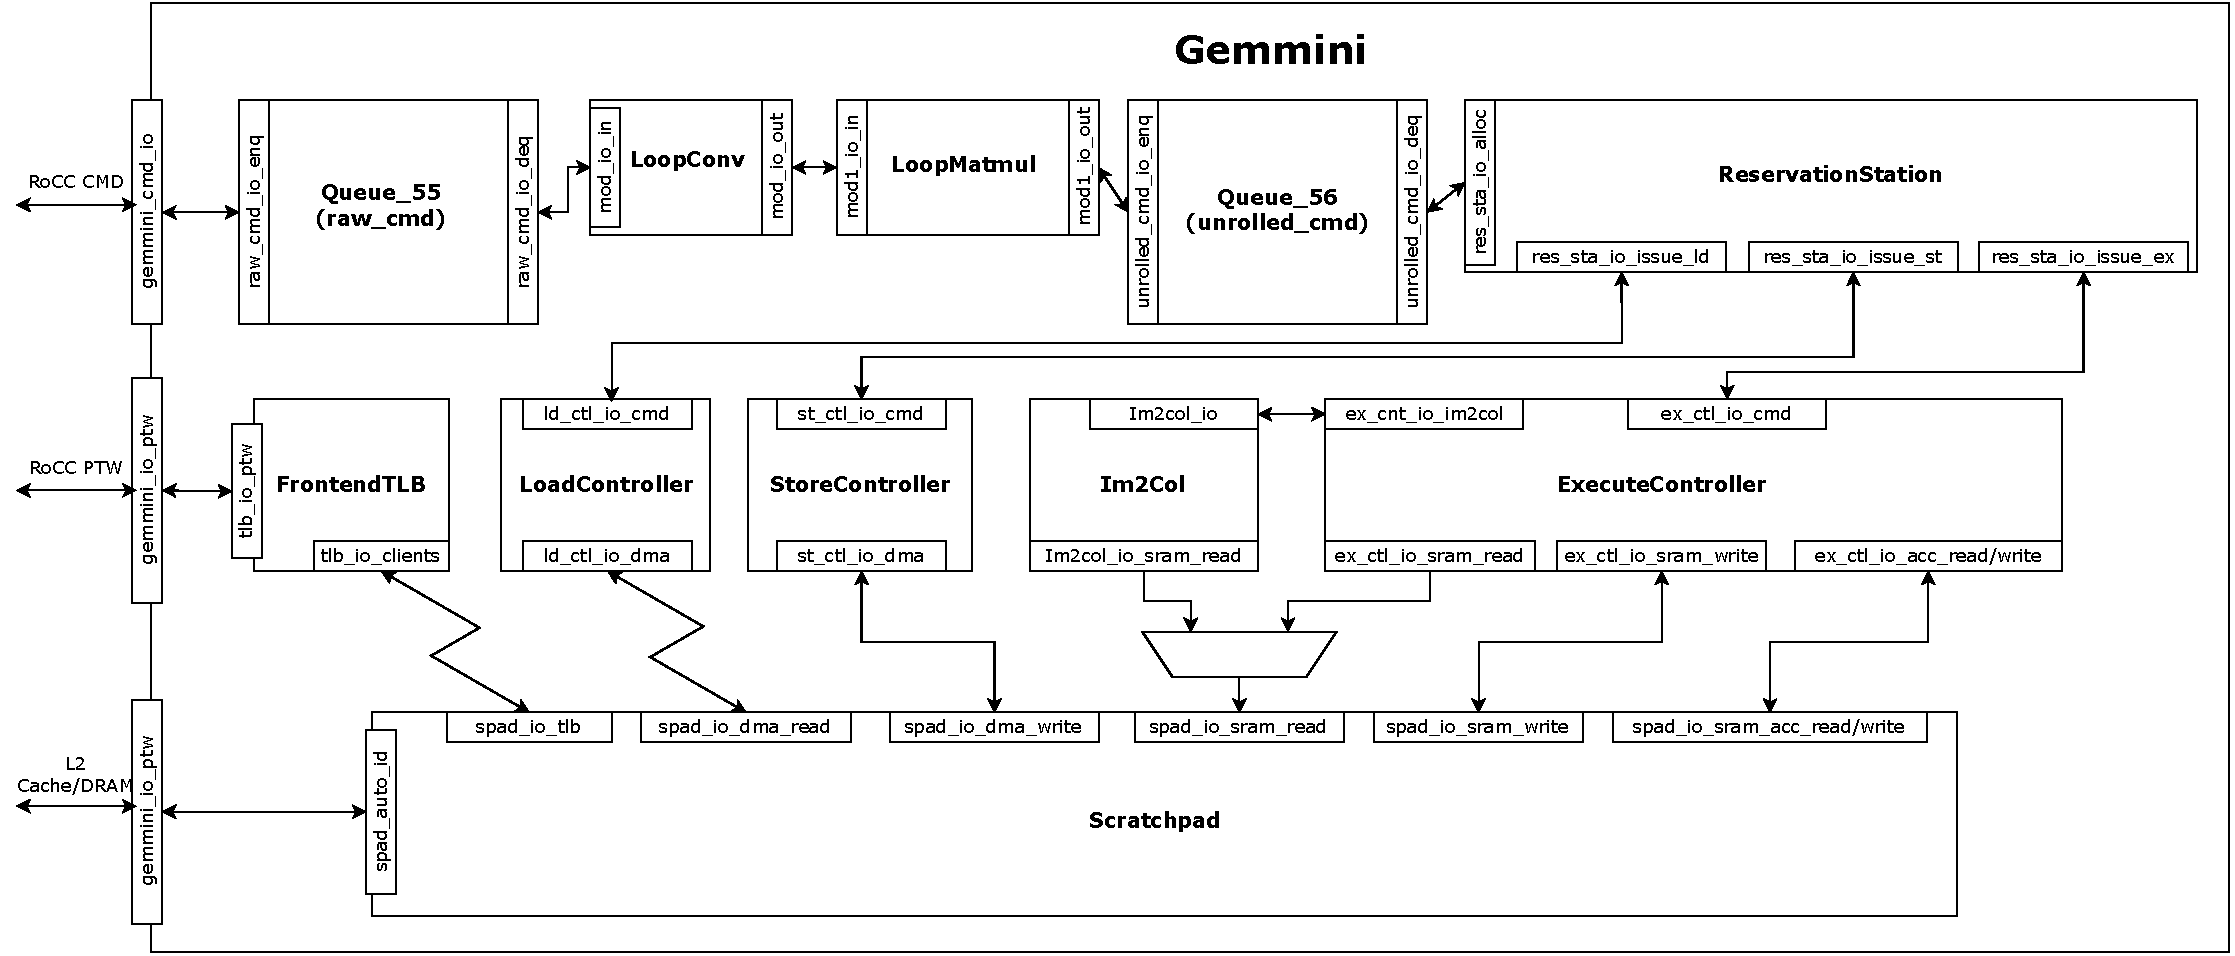
\includegraphics[width=\textwidth]{Gemmini_InternalOverview.pdf}
    \caption{Overview of the internal modules in the generated Gemmini hardware architecture, showing the flow of commands from the RoCC interface through various queues and controllers. Source: \cite{gookyi2023gemmini_case_study}.}
    \label{fig:gemmini_internal_modules}
\end{figure}

\subsection{Command Unrolling and Buffering}
The initial \texttt{RoCC} instructions received from the CPU are often "complex" commands that encapsulate entire loops (e.g., `loop\_matmul`). As shown in Figure~\ref{fig:command_unrollers}, modules like \texttt{LoopMatmul} and \texttt{LoopConv} are responsible for unrolling these high-level tasks into a stream of simpler, primitive micro-operations for loading, storing, and executing on tiled sub-matrices. These primitive commands are then buffered in a queue before being sent to a central dispatcher.

\begin{figure}[htbp]
    \centering
    \includegraphics[width=\textwidth]{_YOUR_IMAGE_PATH_/Sensors_Fig4.png}
    \caption{Gemmini's command unrolling modules (\texttt{LoopConv} and \texttt{LoopMatmul}), which translate high-level commands into a series of primitive operations. Source: \cite{gookyi2023gemmini_case_study}.}
    \label{fig:command_unrollers}
\end{figure}

\subsection{Reservation Station and Execution Control}
The stream of primitive commands is received by the \texttt{ReservationStation} module, which reorders and dispatches them to the appropriate back-end controller. The \texttt{ExecuteController} (Figure~\ref{fig:execute_controller}) manages the actual computation. It issues commands to the systolic array and orchestrates the movement of data between the scratchpad and the computational units. It also contains logic to manage optional units, such as the hardware \texttt{im2col} unit or data transposer.

\begin{figure}[htbp]
    \centering
    \includegraphics[width=\textwidth]{_YOUR_IMAGE_PATH_/Sensors_Fig6.png}
    \caption{The \texttt{ExecuteController} module and its associated SRAM control interfaces. Source: \cite{gookyi2023gemmini_case_study}.}
    \label{fig:execute_controller}
\end{figure}

\subsection{The Mesh and Scratchpad}
The \texttt{ExecuteController} ultimately controls the two lowest-level hardware blocks: the Mesh and the Scratchpad. The Mesh (Figure~\ref{fig:mesh_module}) is the direct hardware implementation of the systolic array, containing the grid of PEs. The Scratchpad (Figure~\ref{fig:scratchpad_module}) implements the on-chip memory, containing the SRAM banks and logic for interfacing with the DMA engine and the systolic array's accumulator.

\begin{figure}[htbp]
    \centering
    \includegraphics[width=0.7\textwidth]{_YOUR_IMAGE_PATH_/Sensors_Fig8.png}
    \caption{The Mesh module, which implements the systolic array of PEs and supports different dataflows (Output Stationary and Weight Stationary). Source: \cite{gookyi2023gemmini_case_study}.}
    \label{fig:mesh_module}
\end{figure}

\begin{figure}[htbp]
    \centering
    \includegraphics[width=\textwidth]{_YOUR_IMAGE_PATH_/Sensors_Fig9.png}
    \caption{The internal structure of the Scratchpad module, showing the various interfaces to the TLB, DMA, and internal memory banks. Source: \cite{gookyi2023gemmini_case_study}.}
    \label{fig:scratchpad_module}
\end{figure}

\section{The Multi-Level Programming Model}
\label{sec:gemmini_programming_model}

To cater to different user needs, from application developers to hardware architects, Gemmini supports a multi-level programming model. This stack provides layers of abstraction, allowing users to work at a level appropriate for their task, from direct hardware control to high-level framework integration.

\subsection{Low-Level: Gemmini ISA}
At the lowest level, Gemmini is controlled by its custom RoCC instruction set. These instructions are typically wrapped in C preprocessor macros for easier use from C/C++ code. The instruction set includes primitive commands like \texttt{mvin} (move data in), \texttt{mvout} (move data out), \texttt{preload} (load data into the PE array), and \texttt{compute}. It also features more "complex" instructions like \texttt{loop\_matmul} that abstract away the manual tiling and scheduling of primitive commands, offloading the loop control to hardware state machines \cite{Genc2022GemminiMLSys}.

\subsection{Mid-Level: Hand-Tuned C Library}
To abstract the complexities of direct ISA programming, Gemmini provides a C library (typically accessed via \texttt{gemmini.h}). This library offers functions for common DNN operations, such as \texttt{tiled\_matmul} and \texttt{tiled\_conv}. These functions implement optimized heuristics for loop tiling and data movement to maximize scratchpad utilization based on the specific hardware parameters of the generated Gemmini instance.

\subsection{High-Level: Compiler Support (Conceptual)}
The Gemmini ecosystem is designed to support higher-level compilation flows. This involves tools that can take DNN models described in standard frameworks like ONNX (Open Neural Network Exchange) and compile them down to Gemmini instructions, either by calling the mid-level C library or by directly generating low-level ISA calls. This further simplifies the deployment of DNNs on Gemmini-accelerated SoCs.

\section{Gemmini Configuration in This Thesis}
\label{sec:gemmini_configuration}

The Gemmini accelerator integrated into the SoC for this thesis is based on a specific configuration suitable for the target AI applications and FPGA resource constraints. Within the Chipyard framework, this configuration is defined in a Scala configuration file. 
\todo[inline]{Specify the key parameters for your Gemmini instance here. For example: The instance was configured with a 16x16 systolic array using 8-bit integer data types for inputs and weights, and a 32-bit integer accumulator. The scratchpad was configured with 256KB of capacity and the accumulator memory with 64KB. The Weight Stationary (WS) dataflow was selected, and the hardware \texttt{im2col} unit was included to offload this pre-processing step from the host CPU. These parameters were chosen to balance performance for target DNN workloads with the resource constraints of the target FPGA. The detailed performance implications of these choices will be explored in subsequent chapters.}

The integration follows the standard \texttt{RoCC} methodology provided by Chipyard, ensuring that Gemmini coexists with the Rocket Core, shares the system memory hierarchy, and can be programmed using custom RISC-V instructions dispatched to its \texttt{RoCC} slot.

% Công trình của tác giả (nếu không có thì comment 02 dòng dưới)
\cleardoublepage
\newpage
\phantomsection
%\addcontentsline{toc}{chapter}{DANH MỤC CÔNG TRÌNH CỦA TÁC GIẢ}
%\include{Appendix/publish}

% In tài liệu tham khảo
\cleardoublepage
\newpage
\phantomsection
\addcontentsline{toc}{chapter}{TÀI LIỆU THAM KHẢO}
\printbibheading[title={TÀI LIỆU THAM KHẢO}]

\printbibliography[heading=subbibliography, title={Tiếng Việt}, keyword=Viet, resetnumbers=true]

\DeclareNameAlias{sortname}{last-first}
%\DeclareNameAlias{default}{last-first}

\printbibliography[heading=subbibliography, title={Tiếng Anh}, notkeyword=Viet, resetnumbers=true] 
% ===================================================================== %
% CHÚ Ý: phải gán lại resetnumbers=số tài liệu tham khảo tiếng Việt + 1 %
% ===================================================================== %

% Phần phụ lục
\appendix

\chapter{MÃ NGUỒN CỦA THIẾT KẾ}
\label{Appendix1}

\section{Mã Verilog Top-Level cho DMANiosV}
\label{app:verilog_top} % Changed label for clarity


\appendix
\renewcommand{\thechapter}{B} % Set Appendix Chapter Label to B

\chapter{MỘT SỐ LỖI THƯỜNG GẶP}
\label{Appendix2}

Phần này bao gồm một số lỗi thường gặp và cách khắc phục trong quá trình triển khai và gỡ lỗi hệ thống Nios V với DMA.

\section{Lỗi Tạo BSP hoặc Biên dịch Ứng dụng}
\label{sec:trouble_bsp_app}

Một lỗi phổ biến khi chạy lệnh \texttt{niosv-app} là báo không tìm thấy tệp hoặc thư mục nguồn.
\begin{itemize}
    \item \textbf{Nguyên nhân:} Đường dẫn đến thư mục \texttt{app}, \texttt{bsp}, hoặc tệp mã nguồn C (\texttt{-s=...}) không chính xác so với vị trí hiện tại (hoặc không tồn tại) của Nios V Shell. 
    \item \textbf{Khắc phục:} Đảm bảo đã \texttt{cd} vào thư mục gốc của dự án Quartus (\texttt{DMANiosVIntern}) trước khi chạy lệnh \texttt{niosv-app}. Kiểm tra lại các đường dẫn tương đối (\texttt{software/app}, \texttt{software/bsp}) trong lệnh. Tên tệp mã nguồn C trong thư mục \texttt{app} phải khớp với tên được chỉ định bởi tham số \texttt{-s}.
\end{itemize}

\end{document} 
